%%%%%%%%%%%%%%%%%%%%%%%%
%% Sample use of the infthesis class to prepare a thesis. This can be used as 
%% a template to produce your own thesis.
%%
%% The title, abstract and so on are taken from Martin Reddy's csthesis class
%% documentation.
%%
%% MEF, October 2002
%%%%%%%%%%%%%%%%%%%%%%%%

%%%%
%% Load the class. Put any options that you want here (see the documentation
%% for the list of options). The following are samples for each type of
%% thesis:
%%
%% Note: you can also specify any of the following options:
%%  logo: put a University of Edinburgh logo onto the title page
%%  frontabs: put the abstract onto the title page
%%  deptreport: produce a title page that fits into a Computer Science
%%      departmental cover [not sure if this actually works]
%%  singlespacing, fullspacing, doublespacing: choose line spacing
%%  oneside, twoside: specify a one-sided or two-sided thesis
%%  10pt, 11pt, 12pt: choose a font size
%%  centrechapter, leftchapter, rightchapter: alignment of chapter headings
%%  sansheadings, normalheadings: headings and captions in sans-serif
%%      (default) or in the same font as the rest of the thesis
%%  [no]listsintoc: put list of figures/tables in table of contents (default:
%%      not)
%%  romanprepages, plainprepages: number the preliminary pages with Roman
%%      numerals (default) or consecutively with the rest of the thesis
%%  parskip: don't indent paragraphs, put a blank line between instead
%%  abbrevs: define a list of useful abbreviations (see documentation)
%%  draft: produce a single-spaced, double-sided thesis with narrow margins
%%
%% For a PhD thesis -- you must also specify a research institute:
%\documentclass[phd,cisa,twoside,logo,parskip]{infthesis}

%% For an MPhil thesis -- also needs an institute
% \documentclass[mphil,ianc]{infthesis}

%% MSc by Research, which also needs an institute
% \documentclass[mscres,irr]{infthesis}

%% Taught MSc -- specify a particular degree instead. If none is specified,
%% "MSc in Informatics" is used.
% \documentclass[msc,cogsci]{infthesis}
 \documentclass[msc]{infthesis}  % for the MSc in Informatics

%% Undergraduate project -- specify the degree course and project type
%% separately
% \documentclass[bsc]{infthesis}
% \course{Artificial Intelligence and Psychology}
% \project{Fourth Year Project Report}

%% Put any \usepackage commands you want to use right here; the following is 
%% an example:
\usepackage[numbers]{natbib}
%\usepackage{hyperref}
\usepackage{graphicx}
\usepackage{amssymb,amsmath}
\usepackage{epstopdf}
\usepackage{parskip}
\usepackage{setspace} 
\usepackage{algorithm}
\usepackage{algpseudocode}
\usepackage{enumitem}
\usepackage{microtype}
\usepackage{mathpazo}
\renewcommand{\rmdefault}{pplx}

%% Information about the title, etc.
\title{Improving The Performance Of  Similarity Metrics Used For Comparing Time Series Sequences}
\author{M. Adnan Haider}

%% If the year of submission is not the current year, uncomment this line and 
%% specify it here:
% \submityear{1785}

%% Optionally, specify the graduation month and year:
% \graduationdate{February 1786}

%% Specify the abstract here.
\abstract{%
    %This doctoral thesis will present the results of my work into the
    %reanimation of lifeless human tissues.
}

%% Now we start with the actual document.
\begin{document}

%% First, the preliminary pages
\begin{preliminary}

%% This creates the title page
\maketitle

%% Acknowledgements
\begin{acknowledgements}
Many thanks to my mummy for the numerous packed lunches; and of course to
Igor, my faithful lab assistant.
\end{acknowledgements}

%% Next we need to have the declaration.
\standarddeclaration

%% Finally, a dedication (this is optional -- uncomment the following line if
%% you want one).
% \dedication{To my mummy.}

%% Create the table of contents
\tableofcontents

%% If you want a list of figures or tables, uncomment the appropriate line(s)
% \listoffigures
% \listoftables

\end{preliminary}

%%%%%%%%
%% Include your chapter files here. See the sample chapter file for the basic
%% format.
 \begin{spacing}{1.25}
\include{chapter1}
\chapter{Introduction}


Over the course of the last decade, the mining of time-series data has received considerable attention within the  data mining and machine learning community. The term 'time series'  represents a  sequence of numerical data points collected at regular intervals over a period of time. The duration of time period may be  either in the order of milliseconds or monthly or even annually depending on the domain. 

Mathematically, a time series is defined by the values $y_1, y_2...y_n$ at times  $t_1,t_2... t_n$  where $y=f(t)$.  The time $t_i$  acts as an independent variable to estimate dependent variables $y_i$. The dimensionality of the  series is denoted as \textbf{n} where the value of  `\textbf{n}' is equal to the length of the sequence. 

 Time series analysis is used in many applications ranging from  sales forecasting, budgetary analysis to stock market analysis and many more. One particular domain where the application of time series analysis is currently very popular is \emph{motif} discovery- the problem of efficiently locating frequent/interesting sub-patterns in the data.  The knowledge of motifs has been seen  to have important applications in various aspects of data mining tasks. For instance motifs can use applied :

 \begin{itemize}
\item  to discover association rules \citep{GautamDas} that the reflect information of `primitive shapes. 
\item to specify the number of clusters for  unsupervised clustering algorithms. The knowledge of motifs give a good approximation on the number of meaningful groups that are present in the data\citep{Fayyad1998}.
\item to identify important sub-patterns in DNA and gene sequences \citep{BRAZMA1998}. 

\end{itemize}



In the analysis of speech data, motifs  also play a very important role. Recent research have shown that detecting and isolating motifs in speech  utterances is equivalent to identifying  words that are specific to genres or  in the case of recordings of individual speakers, detecting  words that  are frequently spoken by them. \citep{Park2008,Zhang2010}. %The methodology proposed in these papers  is based on constructing  a framework that is entirely data driven  i.e there is no intermediate recognition stage  that maps an audio signal to a symbolic representation such as the `phone' states in the HMM model. This  results in   the word acquisition process to be unsupervised which presents a  completely   different approach to the current speech recognition systems that are built using a supervised  training methodology employing  manually transcribed speech to model the underlying speech process.

  
To identify and extract motifs from time series data, various metrics have been proposed to match similar time series sequences. Among them, the most widely used  is the  Dynamic time warping  algorithm(DTW) \citep{Salvador,Sakoe1990,Rabiner1978,Xie2010,Xi2006,Fu2007} which  matches similar sequences separated by time shifts, length or scale. By warping the time axis, the  DTW algorithm  compares each point in one sequence with  points at different temporal regions   in the second sequence.  This allows the algorithm to be invariant to changes of speed, length or scale between similar patterns and thus provide a much richer comparison between time series sequences in comparison to standard metrics such as the Euclidean distance .  Metrics such as the Euclidean distance  are constrained to performing only linear matches between the temporal dimensions of sequences and  require the all sequences to share the same length. This provides a limitation on the type of time series domains such metrics can be applied to.  The speech corpus is an  prime example of one such domain where distance metrics such as the Euclidean cannot be applied directly. In such data sets, recorded utterances of the same same lexical identity may not necessarily share the same  dimensionality (i.e  the same length) and thus may be contracted/expanded versions of each other due to speaker variations, context etc. 

However, the DTW algorithm also experiences from severe drawbacks. The algorithm suffers from large run-times when the length of the time series sequences are very long. This is because  the  time complexity of the algorithm  is quadratic i.e O($n^2$ ) where n is the length of the  sequence.  In comparison, standard metrics like the euclidean  has a time complexity of O(n), making them computational less expensive to employ. To address the  quadratic time complexity of the DTW algorithm  window constraints (Itakura parallelogram\citep{Itakura1975}, Sakoe-Chiba band\citep{Sakoe1990}) have been proposed to  reduce the  size of the search space of DTW  by forcing the algorithm to look for optimal paths that are along the diagonal. Although introducing such window constraints does improve the time complexity, the reduction in the search space however  leads to a substantial decrease in the accuracy of the algorithm since all optimal paths may not exist around the diagonal region\citep{Fu2007}.


The goal of this project is  to employ machine learning techniques to tackle and resolve the individual drawbacks associated with using the DTW algorithm and the euclidean metric  to compute the similarity between high dimensional time series sequences. In the  first half of the project, I will be solely concentrating  on improving the performance of the DTW algorithm for problem domains where the minimising the time complexity is as high priority as achieving good accuracy. In the latter half  of the project, I will be concentrating on improving the  performance of  the  euclidean metric in  time series domains where intra class sequences share the same global shape. To be precise, I will be exploring feature extraction techniques to  extract a smaller set of independent  features from the raw sequences that can  capture information about the global shape and be used by the euclidean metric to cluster/classify intra class sequences that share global trends.
%The discovery of motifs in high dimensional time series data(i.e long sequences) that vary in length  is still a difficult problem to work with. To address the drawbacks of DTW and SVD, there has been some recent work conducted to improve these algorithms. In the paper `` \emph {Fast time series classification using numerosity reduction}", the authors address the drawbacks of DTW in handling high dimensional sequences. They propose an adaptive approach that initially uses a strict window constraint to reduce the search space of DTW but then gradually increase size of the window by discarding samples from the training set. Although this methodology improves the time complexity of the dynamic time warping algorithm by heuristically discarding regions in the input space, the methodology is more tailored to  smart data selection rather than improving the algorithm itself. In the case of SVD, for high dimensional time series sequences which vary in length, the  data matrix  suffers in being  incomplete. Carelessly addressing only the relatively few known entries is highly prone to over �tting. Earlier works [21] relied on imputation to fill  in missing ratings and make the rating matrix dense. However, imputation can be very expensive as it significantly  increases the amount of data. In addition, the data may be considerably distorted due to inaccurate imputation. 

 For this project, I will be primarily using 3 time series datasets (details given in chapter 2):
\begin{itemize}
\item TIDIGITS corpus 
\item InLineSkate
\item Cinc\_ECG\_TORSO
\end{itemize}

 To evaluate and compare the merits of different proposed changes, I have  partitioned each of the above datasets into  a training set and a test set  and employed the 1 nearest neighbour classifier to classify the test instances. In the first half of the project, the DTW was used as the similarity metric while for the later analysis, the euclidean metric was employed as the similarity metric. The performance of the classifier has been used to compare  different proposed adaptions of the DTW and evaluate  the performance of using different feature sets  when employing  the euclidean metric.  The reason for choosing the 1 nearest neighbour classifier is that it shares almost the same methodology as the algorithms used to detect motifs. Motif detection algorithms are memory based i.e like 1NN classifier, they rely on comparing each sequence with other sequences in the dataset. Hence, methodologies that tend to achieve good performance on 1NN classification can be expected to achieve equivalent performance in motif detection. 
 
 
 %However, the 1 nearest neighbour classifier deters from motif detection on two aspects: each sequence in the test set is compared with sequences of the training dataset and not the entire data set. The entire process is supervised i.e correct label information are available to check the accuracy of the algorithm. Secondly, when conducting 1NN classification, each sample is considered as a single motif  but in real motif detection problems a single sample can contain multiple motifs.
 
  %For a majority portion of the analysis, the TIDIGITS corpus will serve as  the primary dataset used  to investigate the performances of different models. The reason being the TIGITS corpus consists  of long time series sequences that vary in length . Since each  time sequence corresponds to a speech utterance spoken by a speaker, as result of environment, context and speaker differences the length of the time series sequences will not be the same. In comparison, the sequences with in each UCR data set share the same dimensionality i.e length. Furthermore, the length of the time series sequences on average is much higher in the TIDIGITS corpus than sequences of any data set in the UCR time series database.Thus the TIDIGITS data set is an ideal choice to investigate  the performance of different models in my project.
 %The discovery of motifs in high dimensional time series data that vary in length  is still a difficult problem to work with. Current works have only tried to address the issue of high-dimensional spaces. The state of the art algorithms have been to designed to work on high-dimensional time series sequences that all share the same length. To my knowledge, there exits no algorithm apart from DTW that can applied to high-dimensional sequences varying in length.  Using this as motivation, the aim of this project is to investigate methods  that can improve the discovery of motifs in  high-dimensional time-series sequences that vary in length. In this project, I particularly focus on improving the performance of the DTW algorithm in high dimensional spaces and in the later chapters investigate on  how to adapt unsupervised parametric models to high dimensional  data sets  that vary in length. 

The  dissertation is  organised as follows: Chapter 2 gives a brief description of the  time-series datasets used for this project. Chapter 4  provides a detailed background description of the DTW algorithm.  Chapter 3 and 4 investigates methods to improve the performance of the DTW algorithm in terms of both accuracy and speed. Chapter 5 explores the novel technique of single value  decomposition in the context of time series domains and explores whether it can be applied to extract a smaller set of latent features that can minimise  the run time of the 1NN classifier when using the euclidean metric to classify sequences. Chapter 6 focusses on improving the accuracy of the classification of 1NN classifier on time series sequences when it employes  the euclidean metric. In this chapter, I mainly explore preprocessing techniques  that can extract novel features which capture the  global properties of sequences.  Finally in the last chapter, I present my conclusions and present scope for future work.

\include{chap3}
\chapter{Datasets Used}
There are  two primary goals of this project : 
\begin{itemize}
\item improve the performance of the DTW  algorithm on long time series sequences. 
\item explore the use of feature extraction methods to generate a small set of descriptive latent  features\citep{Cadzow1983}  that can be used by the euclidean metric to cluster intra class sequences that share global trends more accurately.
\end{itemize}
The performance of the 1 NN classifier has been used to compare different proposed adaptions of the DTW and evaluate the performance of using different feature sets when employing the euclidean metric. For this project,  the datasets used for evaluation were carefully chosen so that they contain time series sequences that have very\textbf{ high} dimensions i.e long lengths.
 
 The datasets used for this project are as follows:
\begin{enumerate}
\item TIDIGITS speech corpus
\item   The UCR data set :CinC\_ECG\_torso
\item The UCR data set :InlineSkate
\end{enumerate}
All 3 data sets were partitioned into two disjoints sets: test set and training sets. Each sample in the training and test data set corresponds to a particular pattern. The class information of the training samples were used to evaluate the accuracy of the nearest neighbours classifier.

For the first half of the project, the primary dataset that was mostly used is the `TIDIGITS' corpus. In comparison to the sequences in the two UCR datasets, the length of the time series sequences in the TIDIGITS corpus are on average 100 times longer. This forces the DTW algorithm to suffer from high time complexity when handling the speech utterances.  The TIDIGITS corpus is a prime example where the minimisation of the run time is as high priority as getting good accuracy. In chapter 4 and 5, I will be investigating domain dependent and independent methodologies to improve the performance of the DTW in high dimensional time series datasets such as the TIDIGITS corpus. 

The TIDIGITS corpus consists of time series sequences that are of variable length. Since the application of the euclidean metric is restricted to time series sequences  that share the same length, for the later half of the project, I will be focussing mainly on the UCR datasets when exploring the use of various feature extraction methods that can improve the accuracy of the Euclidean metric in computing the similarity between intra class sequences that share the same length.

Description of the data sets is given below:
\section { Brief description of TIDIGITS dataset}
The TIDIGITS dataset is a large speech database  that has been collected for the  use in designing and evaluating algorithms for speaker-independent recognition of connected digit sequences. This dialectically balanced database consists of more than 25 thousand digit sequences spoken by over 300 men, women, and children. The data were collected in a quiet environment and digitised at 20 kHz\citep{TIDIGITS}. The vocabulary of the corpus consists of :
\begin{itemize}
\item 22 isolated digits (two tokens of each of the eleven digits)
\item 11 two-digit sequences
\item 11 three-digit sequences
\item 11 four-digit sequences
\item  11 five-digit sequences
\item  11 seven-digit sequences
\end{itemize}
In this corpus, the motifs correspond to individual digits. Thus for my experiments, I have considered  only the  isolated digit sequences for classification,  more specifically the digits from 0 to 9. The database was divided into two subsets, one to be used for algorithm design and one to be used only for evaluation. The division was based on speaker category $\{men,women,boy,girl\}$ and dialect classification, and yielded two sets of speakers, each containing approximately half the speakers of each category.

 The table below shows the partitioning of speakers from different speaker categories in the training and test dataset.:

\begin{tabular}{|c|c|c|c|c|}
\hline \\
Subset  &    Man &   Woman &Boy &   Girl  \\
         Train &         55&     57 &  25 &     26\\
    
         Test      &     56 &    57 &   25 &     25\\
 \hline
 \end{tabular}

For this project, only samples from one production have been used. To perform 1 NN classification, the entire training set have been used . However,  to ensure that the experiments completed with in a reasonable time, I have only used $\frac{1}{3}$ of the samples of the test set.

The test data subset used for evaluation consists of 
\begin{itemize}
\item 162 random samples from boy category
\item 162 random samples from girl category
\item 326 random samples from men category
\item326 random samples from women category
\end{itemize}
\textbf{Note}: The samples were not  chosen exactly randomly. When subsampling from each category, I have ensured that:
\begin{itemize}
\item  the test set contained samples from a rich variety  of  different speakers. 
\item  the chosen subset consists of  enough examples of all 10 digits.
\end{itemize}
  
\section{Brief description CinC\_ECG\_torso and InLineSkate dataset}
The UCR data resource  has been  funded by an NSF(National Science Foundation) since 2003 and is the largest public collection of time series data sets that have been made available to the data mining/machine learning community, to encourage reproducible research for time series classification and clustering.  

The InLineSkate dataset represents the EMG data of 7 major leg extensor and flexor muscles of the right side of the body from six athletes collected  by attaching  bipolar surface electrodes to the relevant muscles\citep{Morchen2006}.The sampling rate was 1 kHz. The Cinc\_ECG\_Torso presents the ECG data collected by attaching  electrodes to 4 distinct regions on the torso  from  multiple participants.

\textbf{InLineSkate}:
  \begin{itemize}
    \item Length of the time series:1882
  \item Size of test set:550
  \item Size of training set:100
  \item Number of classes:7 
   \end{itemize}
   \textbf{CinC\_ECG\_torso}:
  
  \begin{itemize}
    \item Length of the time series:1639
  \item Size of test set:1380
  \item Size of training set:40
  \item Number of classes:4
  \end{itemize}
  
\section{Evaluation}
The focus of this project is investigate methods to improve the performance of  the DTW and the Euclidean metric in time series  problem domains where minimising the time complexity is as important as improving accuracy. To evaluate and compare the merits of different proposed methods to improve the accuracy and the computational cost in  comparing time series sequences when using the DTW or the Euclidean distance,  the accuracy and  time incurred by the 1NN classifier to classify all the instances in the respective test sets has been  used as an evaluation criteria. As I have already mentioned in the previous chapter, motif detection algorithms like 1 NN  are memory based i.e each sequence is compared with all sequences in the dataset. Thus, methods that improve  the performance of  the DTW and the Euclidean metrics in classifying sequences that have high dimensionality can be expected to improve the performance of these metrics in detecting motifs in high dimensional time series datasets.


  \include{chap2}

\chapter{Background}
\section {Dynamic Time Warping Algorithm}

The Dynamic Time Warping algorithm is  a distance metric that computes the similarity between  time series sequences varying in length, scale and speed. The problem formulation \citep{Salvador} of the algorithm is stated as follows: Given two time series X, and Y, of lengths $|X|$ and $|Y|$,
\begin{eqnarray}
X &= &x_1,x_2...x_{|X|}\\
Y &= &y_1,y_2...y_{|Y|}
\end{eqnarray}
construct a warping path W
\[ W =  w_1, w_2...w_k \mbox{ where max } (|X|,|Y|)\leq k\leq |X|+|Y|\]
where
\begin{itemize}
\item \emph{k} denotes the length of the warping path 
\item the  mth element of the warping path is $w_m = (i,j) \in [1 : N]\times[1 : M] \mbox{ for } l \in [1 : k]$ where $i$ is an index from the  time series X and $j$ is an index from the time series Y.
\end{itemize}
To  properly understand the above formulation some key definitions must be stated:
 \begin {enumerate}
\item Warping path \citep{Keogh2004}:
An (N,M)-warping path (or simply referred to as warping path if N and M are clear from the context) is a sequence $w= (w_1,...,w_k)$ with $w_l = (i,j) \in [1 : N]\times[1 : M] \mbox{ for } l \in [1 : k]$ that satisfies the following three conditions.
 \begin{enumerate}
 \item Boundary condition \citep{Keogh2004,Sakoe1990,Xi2006,Itakura1975}:  $w_1 = (1,1)$ and $w_k = (N,M)$.

 The boundary condition enforces that the first elements of the series X and Y as well as the last elements of the series X and Y have to be aligned with each other. This prevents the alignment from missing any points.
 \item Monotonicity condition \citep{Keogh2004,Sakoe1990,Itakura1975}: 
 
 $\forall i \in [1:k-1] , [|w_{i+1}-w_{i}|= 1]$. In other words, $ w_k =(i,j), w_{k+1} =(i',j'), i\leq i' \leq i+1, j\leq j'\leq j +1$
 
 The condition requires that  the path will not turn back on itself. Both the i and j indexes either stay the same or increase but they will never decrease. 
 
 \item Step-size condition  \citep{Keogh2004,Sakoe1990,Itakura1975}: $w_{l+1}-w_l \in \{(1,0),(0,1),(1,1)\}$,  $ \forall l \in$ [1:k-1].
 
 The step size condition expresses a kind of continuity condition: no element in X and Y can be omitted and there are no replications in the alignment
 \end {enumerate}
 
 Intuitively speaking, the (N,M) warping path $ w = (w_1,...,w_k) $ defines an alignment  between two sequences $X = (x_1,x_2,...,x_N)$ and $Y = (y_1,y_2,...,y_M)$  by assigning each element of X to a unique element  in Y.   

 \item Optimum Warping Path \citep{Xi2006, Keogh2004}:
 
 The optimal warp path corresponds to the  minimum-distance warp path, where the distance of a warp path W is given as 
 \[ Dist(W) = \sum_{m=1}^{K} dist(X,Y)_{|(w_m)}\]
 where $w_m = (i,j)  \in [1 : N]\times[1 : M]$
 
 The $dist(X,Y)_{|(w_m)}$  represents the distance computed using an appropriate  cost function between the value $x_{i}$ of sequence X and the value $y_{j}$ of sequence Y. 
 \[\emph dist(X,Y)_{|(w_m)} = dist(x_{x_i},y_{y_j}) \]
 
\end{enumerate}
The goal of the DTW algorithm is to compute the distance of the optimal warping path for  given two time series sequences. Instead of attempting to solve the entire problem all at once, the  algorithm utilises the technique of dynamic programming to find an optimum alignment between two sequences through the computation of local distances between the points in the temporal sequences. The algorithm proceeds by  iteratively filling in values for each cell (i,j) in  the  $|X|$ by $|Y|$ cost matrix \emph{D}. The value of the cell (i,j) is given by  $D(x_{i}, y_{j})$  which corresponds to a cost metric $Dist(i,j) $ to compute the distance of  optimum warp path from (1,1) to (i,j) :
\[D(i,j) =Dist(i,j) +min(D(i-1,j),D(i-1,j-1),D(i,j-1))\]
computed using  a cost metric $Dist(i,j) $  
The figure below illustrates the working of the DTW algorithm.
\begin{figure}[H]
  \centering
   
     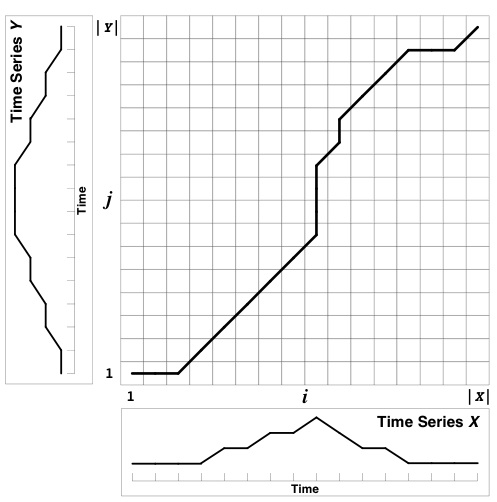
\includegraphics[scale=0.8]{DTWpicture.jpg}
  \caption{The DTW cost matrix with the minimum-distance warp path traced through it.  }
  \end{figure}
Generally the Euclidean metric is widely used as a cost metric. For comparing individual points between time series sequences, the metric is defined as: $Dist(i,j) = (x_i-y_j)^2$ .  For this project, I will be thus considering the DTW algorithm equipped with the euclidean metric as my baseline \textbf{DTW algorithm}. An outline of the base line  DTW algorithm is given below:

 \begin{algorithm}[H]

\begin{algorithmic}[1]
\Procedure{Base line DTW}{$seq1,seq2$}\Comment{two raw sequences }
\State DTW= zeros(length(seq1)+1,length(seq2)+1)
 \For{i=1: to length(seq1) }\Comment{Initialise the DTW cost matrix}
 \State DTW(i,0) = $\infty$
 \EndFor
 
 \For{i=1 to length(seq2)}
 \State DTW(0,i) = $\infty$
 \EndFor
 
  \For{i=2 to length(seq1)}  
 \For{j=2 to length(seq2)} \Comment { cost(a,b)$\equiv$euclid(a,b)}
 \State DTW(i,j) = cost(seq1(i),seq2(j)) + min\{ DTW(i-1,j)+DTW(i,j-1)+DTW(i-1,j-1)\}
 \EndFor
 
 \EndFor
\State \textbf{return}  result = $\frac{\mbox{DTW(n,m)}}{nm}$ \Comment{n=length(seq1), m=length(seq2)}

\EndProcedure 
\end{algorithmic}
\caption{Base line DTW}
\end{algorithm}

  The computational complexity of the DTW algorithm is \emph{O}($n^2$) where $n$ denotes the length of the sequences that are being compared. Thus for time series domains having high dimensions i.e. long lengths, the time and computational costs incurred by the algorithm are quite high.  To address this issue, two well-known global window constraints are employed:  the Sakoe-Chiba band \citep{Sakoe1990} and
the Itakura parallelogram \citep{Itakura1975} . Figure 3.2  gives an illustration  of the use of both constraints:
  \begin{figure}[H]
  \centering
   
     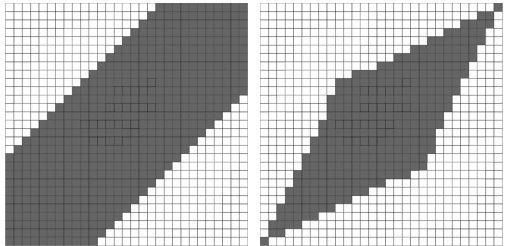
\includegraphics[scale=0.8]{windowconstraint.jpg}
     \caption{ Two constraints: Sakoe-Chuba Band (left) and an Itakura Parallelogram (right), both have a width of 5.}
    \end{figure}
 The shaded areas in the above figure represent the cells of the cost matrix that are filled in by the DTW algorithm for each constraint. The width of each shaded area/window, is specified by a  window parameter. When these constraints are used, the DTW algorithm finds the optimal warp path only through the constraint window. However, the globally optimal warp path will not be found if it is not entirely inside the window\citep{Salvador}. The window parameter therefore determines the accuracy of the DTW algorithm. Decreasing the width decreases the accuracy. If the width is 0 and the series are of equal length then the DTW generalises to the Euclidean distance which is a notoriously inaccurate similarity measure for time series data\citep{Vlachos2002}. To constraint the time complexity to a minimum, the vast majority of the data mining researchers use a Sakoe-Chiba Band with a 10\% width. This reduces the time complexity from O($n^2$) to O (wn) where w is the size of the window parameter. For finding motifs in datasets  comprising of speech utterances, the use of such rigid window constraints is not always desirable. As a result of the same lexical identities spoken in difference contexts, by different speakers, in different environments etc, the optimal alignment paths may not always lie within the regions bounded by the widow constraints\citep{Park2008}.  Thus it is necessary to explore alternative techniques to window constraints that can reduce the time complexity of DTW without degrading its accuracy. In the following chapter, I explore domain-dependent preprocessing methods to improve the performance of the DTW algorithm.

 
  
  \include{chap3}
\chapter{Domain-dependent methods for improving DTW}
%The Dynamic Time Warping(DTW) algorithm is the one of the oldest algorithm that is used to compare and cluster sequences varying in time, scale and speed. Given two temporal sequences, the algorithm utilises the technique of dynamic programming to compute the cost of the optimum alignment path between them.  The computed cost gives an indication of the degree of similarity. The smaller the cost, the more similar the sequences are. Intuitively speaking, DTW can be seen as  a clustering algorithm that clusters patterns that share roughly the same shape. As I have stated in the previous chapter, the time and computational complexity of this algorithm is  \emph{O}($n^2$) where $n$ denotes the length of the sequences that are being compared. Thus for time series domains having high dimensions i.e long sequences, DTW becomes a very unattractive choice as it suffers from high computational and time costs. 

%To address the issue of the curse of dimensionality, DTW algorithms employ a window constraint to reduce the search space. The most commonly used  are Sakoe-Chuba Band\citep{Sakoe1990}  and the Itakura  window constraint \citep{Itakura1975}. Figure[3.2]  gives an illustration of the nature of these window constraints. Such constraints determine the allowable  shapes that a warping path can take by restricting the DTW to construct optimal warping paths only through a restricted number of cells around the diagonal region of the cost matrix. As the dimensionality(length) of the sequences increases, the size of the window is adjusted accordingly. Rigid  window constraints impose a more rigid alignment  that prevent an overly temporal skew between two sequences, by keeping frames of one sequence  from getting too far from the other. The vast majority of the data mining researchers use a Sakoe-Chiba Band with a 10\% width for the global constraint \citep{ChotiratAnnRatanamahatana} to constraint the time complexity of DTW to a minimum. For finding motifs in datasets  comprising of speech utterances, the use of rigid window constraints is highly undesirable. Utterances corresponding to the same lexical identity may suffer from large variations in speed, scale and time due to  the word(s) being spoken in difference contexts, by different speakers, in different environments etc.Thus it is necessary to explore alternative techniques to window constraints that can reduce the time complexity of DTW without degrading its accuracy.

Before investigating methods to improve the DTW algorithm itself, it is highly necessary to first understand the nature of the data sequences that the DTW is presented with.  Achieving a thorough understanding of the data can result in the extraction of a smaller set of relevant features that can be used to achieve better discrimination between different classes/motifs. In this chapter, I investigate domain-dependent preprocessing techniques to improve the performance of the baseline DTW algorithms in clustering patterns that have long lengths.

There are presently two groups of preprocessing techniques commonly used to address this issue:
\begin{itemize}
\item  Feature Selection 
\item Feature Extraction
\end{itemize}
 Feature selection techniques  involve selecting only a subset of attributes from the original data. With respect to the time series data, the technique is analogous to sub-sampling the sequence. To remove redundant features, one of the most popular feature selection approach is  the exploratory data analysis(EDA). EDA is an approach to data analysis that postpones the usual assumptions about what kind of model the data follows with the more direct approach of allowing the data itself to reveal its underlying structure and models. The particular techniques employed in EDA are often quite simple, consisting of various techniques of:
 
 \begin{enumerate}
\item Plotting the raw data such as data traces, histograms, histograms, probability plots, lag plots, block plots, and Youden plots.
\item Plotting simple statistics such as mean plots, standard deviation plots, box plots, and main effects plots of the raw data.
\item Positioning such plots so as to maximise our natural pattern-recognition abilities, such as using multiple plots per page.
 \end{enumerate}
Apart from removing redundant features, we can also construct more useful features from the existing ones. Feature extraction processes are concerned with  the range of techniques  that apply an appropriate functional mapping to the original attributes to extract new features. The intuition behind feature extraction is that the data vectors $\{x_n\}$ typically lie close to a non- linear manifold whose intrinsic dimensionality is smaller than that of the input space as a result of strong correlations between the input features. Hence by using appropriate functional mapping, we obtain a smaller set of features that capture the intrinsic correlation between the input features. By doing so, we move from working in high dimensional spaces to working in low dimensional spaces. The choice  of appropriate functional mapping can  also improve the clustering of data. For example, lets consider figure 4.1: The left- hand plot represents the locations of two dimensional  data points  in the original input space. The colours red and blue denote the classes to which the data points belong to. To cluster the data with respect to their classes, it will be ideal if we can partition the input space into disjoint regions where  intra class variation is small and inter class separation in large. For this example, this is achieved by mapping the points to a feature space spanned by  two gaussian basis functions(shown on the right). Now, we can partition the feature space into two disjoint regions, one of each cluster. 
\begin{figure}[H]
  \centering
   
     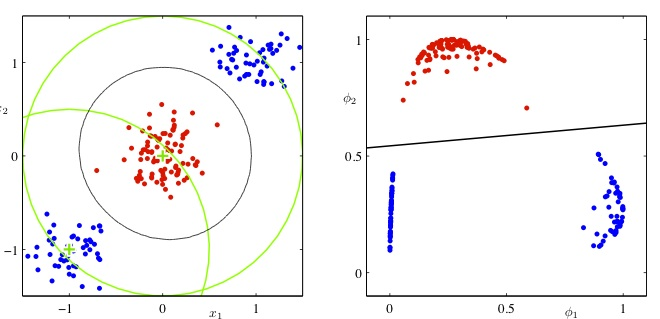
\includegraphics[scale=0.8]{featuremapping.jpg}
  \caption{The figure on the right corresponds to location of the data points in the feature space spanned by gaussian basis functions $\phi_1(x)$ and $\phi_2(x)$ }
  
\end{figure}
In the following sections, I investigate whether the  application of exploratory data analysis and the construction of features that integrate metadata  mainly knowledge of the domain  can aid the baseline DTW algorithm is achieving low run times and good accuracy on long time series sequences. The primary data set that I will be using is the TIDIGITS corpus as the time series sequences of this dataset have lengths that are in the order of $10^4$.
%The DTW algorithm combined  with the  1 nearest neighbour classifier  is a memory based algorithm. Memory-based methods involve storing the entire training set in order to make predictions for future data points. They typically require a metric to be defined that measures the similarity of any two vectors in input space, and are generally fast to �train� but slow at making predictions for test data points. The time and computational complexity associated with such methods is even higher when the dimensionality of the data points is high. Intuitively speaking, DTW is a clustering algorithm that clusters similar patterns varying in time and speed. In high- dimensional spaces, however, the contrast between the nearest and furthest points gets increasingly smaller, making it difficult to construct meaningful cluster groups. To address this issue, data dimensionality methods are used at the  preprocessing stage.
 
\section{Feature Selection}
The computational and time complexity associated with the DTW algorithm is governed by the length of the time  series. Removing redundant features can result in a great reduction in the time complexity without any negative impact on the  accuracy. To get an idea about the underlying structure of the data, I studied the plots of the time series sequences along with listening to the individual samples. Figure 4.2 shows the plot of raw signal corresponding to the word `8' by a speaker from the \emph{boy} category. 


From the visual and auditory analysis, I have made the following  observations:
\begin{itemize}
\item Long durations of silence occupy the beginning and end of each utterance.   The durations of the interesting regions that actually contain information about the spoken digit is quite small is comparison to the durations of silence regions.  Removing these silence segments allow  reduction in the dimensionality of the time series sequences with minimal loss of information.
\item The recordings are highly distorted when played in \emph{matlab}. The distorted signals fail to provide any type of auditory clue about category of the speaker i.e whether the speaker belongs to \{ boy,girl, men,women\} the signal has to be played multiple time to correctly identify the spoken word.
\end{itemize}
\begin{figure}[H]
  \centering
   
     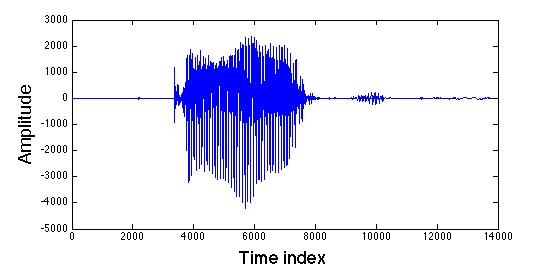
\includegraphics[scale=0.6]{Rawsample.jpg}
  \caption{`Raw 'signal}
  
\end{figure}
\subsection{Signal Filter}
 To remove the redundant attributes from the time series utterances, I have constructed  the following algorithm: `SignalFilter' that performs feature selection by removing segments corresponding to durations of silence.  An outline of the algorithm is as follows:

\begin{algorithm}[h]

\begin{algorithmic}[1]
\Procedure{Signalfilter}{$signal$}\Comment{raw signal }
\State $threshold=0$
\State maxAmplitude= max(rawSignal)
 \State Adapt the threshold based on the value taken by the maximum amplitude
 \State output$\leftarrow$ removeSilence(rawSignal,threshold)
 \State \textbf{return} output%$\leftarrow$ downsample s\_R by $\frac{1}{2}$
 
 \EndProcedure
\end{algorithmic}
 \caption{SignalFilter}
\end{algorithm} 
  The algorithm  employes an adaptive threshold to select and remove redundant attributes. The value of the threshold is dependent on the maximum amplitude of the sequence. The value set is comparatively higher for utterances of speakers having a loud and deep voice and lower for utterances for speakers having gentle and low voice.
  
  
  
 \begin{figure}[H]
  \centering
   
     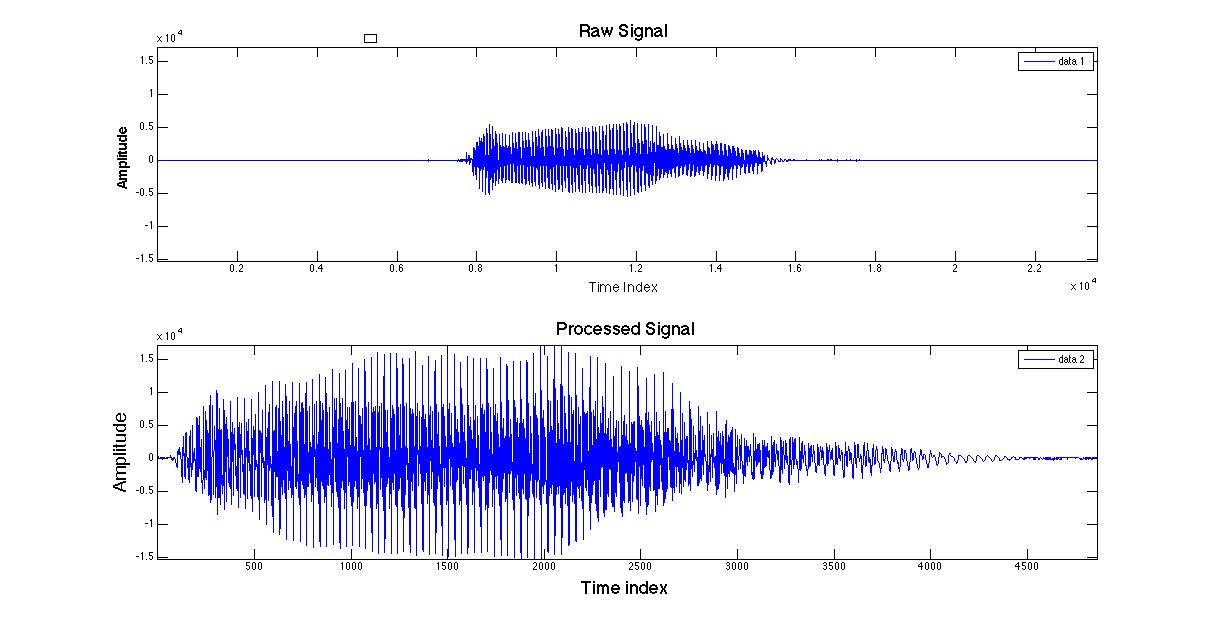
\includegraphics[scale=0.5]{Feature_selection.jpg}
  \caption{shows the raw acoustic signal corresponding to the utterances of the digit '8' alongside with the filtered signal at the bottom.    }
  \end{figure}
 From figure 4.3, it can be observed that the filter preserves the interesting patterns associated with the utterance while succeeding in reducing the dimensionality of the data. To investigate the effect of  introducing this prior feature selection step  on the  performance of the baseline DTW algorithm, I conducted the following experiment:

\textbf{SETUP}: 
 \begin{itemize}
 \item Dataset used: TIDIGITS
 Test-set size : 976 samples

\begin{center} 
 \begin{tabular}{lclcl}
 \hline 
 category &  sample size \\
 boy & 162 \\
 girl & 162\\
 men & 326 \\
 women & 326 \\
 \hline
 \end{tabular}
  \end{center}
  Training  data set size: 1467
  
 \begin{center}
 \begin{tabular}{lclcl}
 \hline 
 category &  sample size \\
 boy & 225 \\
 girl & 234\\
 men & 495 \\
 women & 513 \\
  \end{tabular}
  \end{center}
  
  \item \textbf{Objective}: Investigating the effect of removing silence regions from the raw utterances on the accuracy and run time of the 1NN classifier using the base line DTW algorithm.
  
  \item \textbf{Algorithm:}
  
  The  main objective of my research is to improve the accuracy of the DTW algorithm while reducing the time and computational cost to a \textbf{ minimum}. Even after applying the feature selection process, from initial experiments on few samples, I have found that the computational cost incurred by the algorithm is still very high. Hence to minimise the run time, I  employed the Sakoe-Chuba band that has an adaptive   window size of  : w = max($\lceil{0.1*max(n.m)}\rceil$, abs(n-m)). 
  
  The lower bound of the window size is set to 10\%   of the size of the longest sequence which is the standard width used by the  vast majority of the data mining researchers \citep{ChotiratAnnRatanamahatana}   to keep the time complexity of DTW to a minimum.
  
  An outline of   DTW  algorithm augmented with the adaptive window constraint is given below:
  
   \begin{algorithm}[H]

\begin{algorithmic}[1]
\Procedure{Value-based}{$seq1,seq2$}\Comment{two raw sequences }
\State DTW= zeros(length(seq1)+1,length(seq2)+1)
 \State w = max($\lceil{0.1*max(n.m)}\rceil$, abs(n-m)) \Comment{Window constraint }
 \For{i=1: to length(seq1) }\Comment{Initialise the DTW cost matrix}
 \State DTW(i,0) = $\infty$
 \EndFor
 
 \For{i=1 to length(seq2)}
 \State DTW(0,i) = $\infty$
 \EndFor
 
  \For{i=2 to length(seq1)}  
 \For{j=max(2, i-w) to min(length(seq2), i+w)} \Comment { cost(a,b)$\equiv$euclid(a,b)}
 \State DTW(i,j) = cost(seq1(i),seq2(j)) + min\{ DTW(i-1,j)+DTW(i,j-1)+DTW(i-1,j-1)\}
 \EndFor
 
 \EndFor
\State \textbf{return}  result = $\frac{\mbox{DTW(n,m)}}{nm}$ \Comment{n=length(seq1), m=length(seq2)}

\EndProcedure 
\end{algorithmic}
\caption{Value-Based DTW}
\end{algorithm}

\item RESULTS:

 \begin{figure}[H]
   \centering
   
     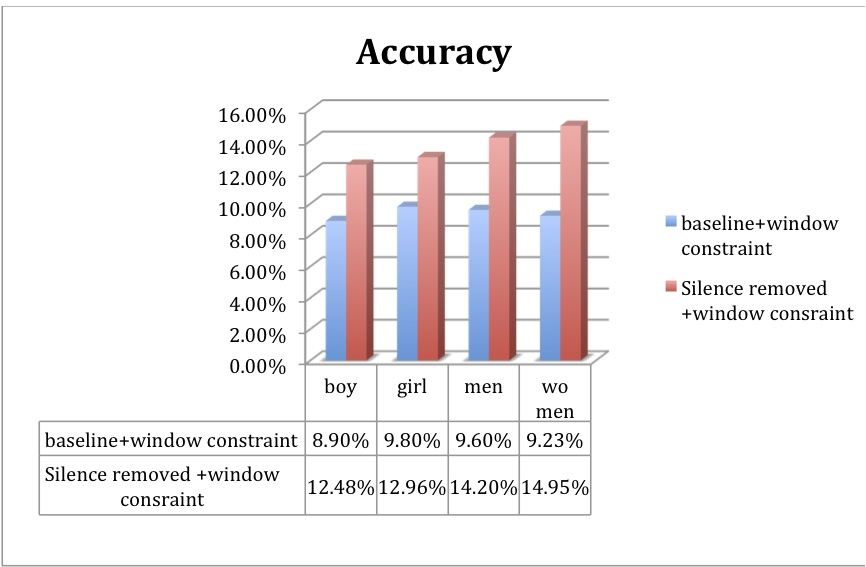
\includegraphics[scale=0.8]{4111.jpg}
  \caption{ }
  
\end{figure}
\begin{figure}[H]
  \centering
   
     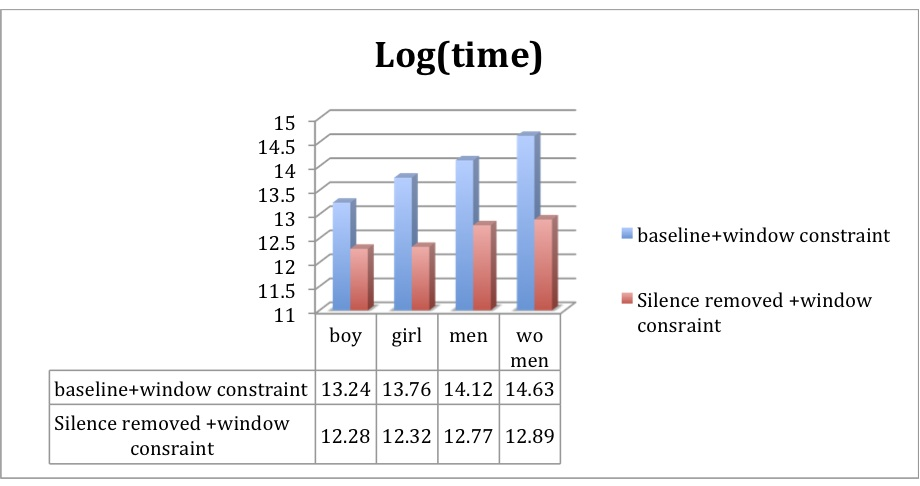
\includegraphics[scale=0.7]{4112.jpg}
  \caption{}
  
\end{figure}
\end{itemize}
Observations:
\begin{itemize}

\item The  DTW algorithm achieves very poor accuracy. The poor accuracy is a result of one  or  a combination of the following three factors:
\begin{itemize}
\renewcommand{\labelitemi}{$\rightarrow$}
\item the use of raw values a features: the numerical value associated with each time point is not a complete picture of the data point in relation to the rest of the sequence.
\item the use of the rigid window constraint- the  low accuracy may be attributed to the optimum warping path between similar patterns lying outside boundaries of the Sakoe-Chuba bands\citep{Zhang2010,Park2008}.
\item not integrating knowledge of the domain: The data set is comprised of speech utterances. It is a widely known fact that for speech data, the MFCC feature vectors capture the information of phones that make up a word. Since different lexical identities are composed of different phones, these use of MFCC vectors can increase the inter class variance of the samples. (details of MFCC to follow)\citep{Park2008,DeWachter2007,Zhang2010,DeWachter2004,Carlin}.
 \end{itemize}

 \item Removing `silence' segments improve \textbf{both} the accuracy and the run-time of the algorithm. While the reason for the decrease in run-time is quite obvious, the increase in accuracy is not. All utterances contain durations of silence. Including the silence regions decreases the inter class variance and in turn increase intra class variance as  they bring in an unwanted notion of similarity in dissimilar patterns.
 
\end {itemize}

\subsection{Downsampling}
From conducting further exploratory data analysis,  I have observed that if  I down-sample the utterances by $\frac{1}{2}$  which in other words corresponds to decreasing the sampling frequency by half, the global shape is still preserved  even though some local information is lost as shown in figure 4.6. This results in further reduction in the dimensionality of the sequences i.e the length of the sequences. 

 \begin{figure}[H]

    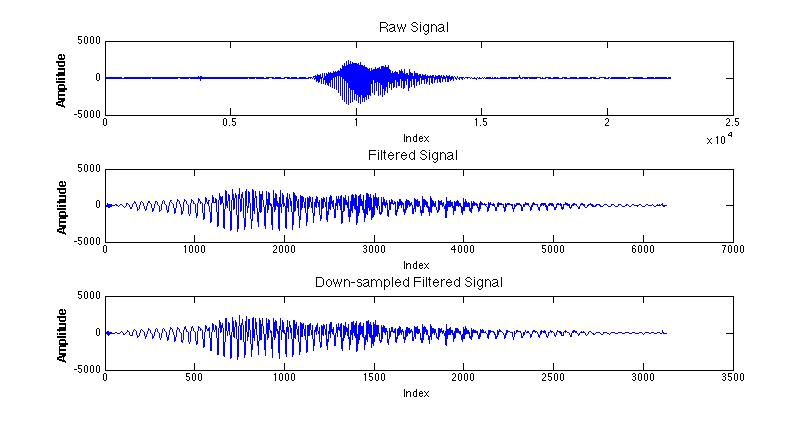
\includegraphics[scale=0.4]{Feature_selection2.jpg}
  \caption{shows the raw acoustic signal of the digit `8' (top figure), the silence removed version of the signal(middle) and the silence removed and down sampled version of the acoustic signal (bottom) }
  \end{figure}
To investigate  the effect of performing further dimensionality reduction on the time series sequences through down sampling on the accuracy of the DTW, I performed the following experiment:

\textbf{Dataset}: The TIDIGITS training and set used in 4.1.1\\
\textbf{Algorithm} : baseline DTW augmented with an adaptive window constraint(4.1.1)
\textbf{Approaches being compared}: Removing silence utterances which we denote as method \textbf{M1}  VS  Removing silence utterance + downsampling VS baseline which we denote as method \textbf{M2}.

\textbf{Results}:
\begin{figure}[H]
 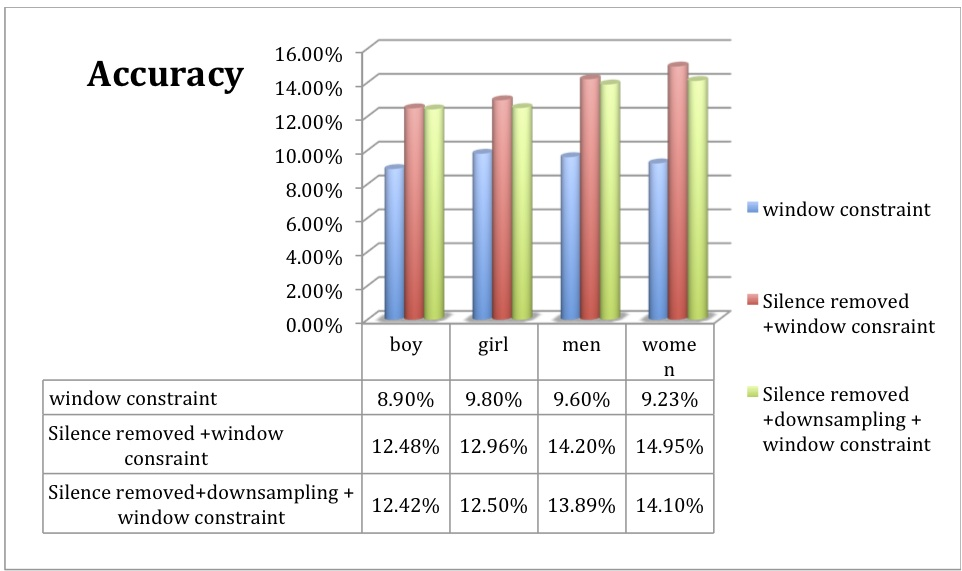
\includegraphics[scale=0.7]{4121.jpg}
  \caption{ }
  \end{figure}
  Observations:
  
 Performing the two stage feature selection step that involves removing `silence' utterances followed by downsampling allow DTW to still  construct more optimal paths that are aligned along the main diagonal for similar patterns than using the entire `raw' time series sequences.  This procedure results in  a 4\% increase in  accuracy on average. Furthermore,  the loss of local information through downsampling the non-silence regions leads to a minimal decrease in the accuracy of the algorithm in comparison to using  the entire non silence regions for pattern matching.  This supports the claim that the classes  are differentiated mainly  by their global shape.  
  
 \begin{figure}[H]
  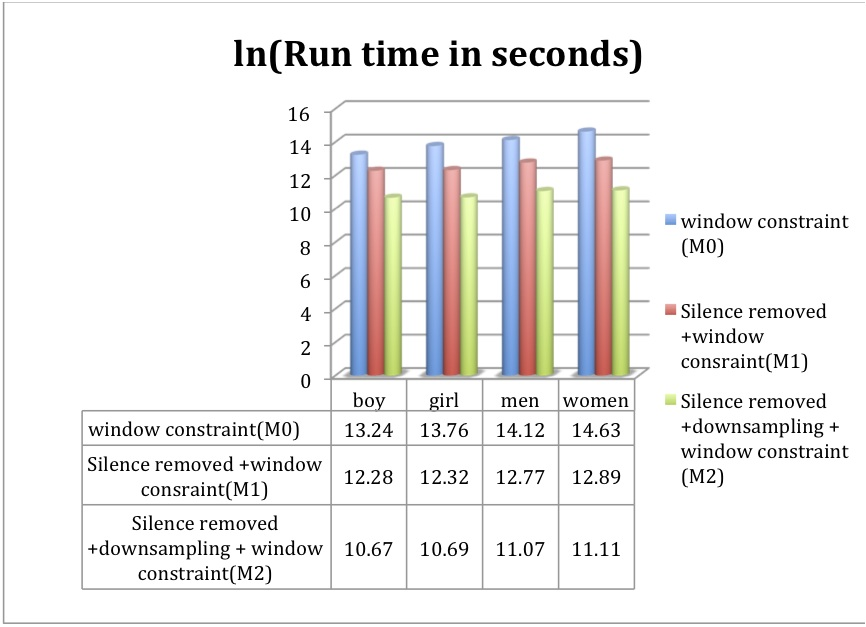
\includegraphics[scale=0.7]{4122.jpg}
     
  \caption{ Integrating downsampling  decreases the ln of the run time that is measured in seconds}
\end{figure}
Augmenting the down sampling procedure to the feature selection process leads to a further decrease of 1.5  in the ln( run time) of the DTW algorithm in comparison to just removing silence regions as a preprocessing step. This is expected since in the first stage of the preprocessing phase, redundant features are dropped which reduces the dimensionality(i.e length ) of the sequences. The length of the sequences is reduced even further through downsampling the the output sequences of stage 1. Since the computational cost of DTW is directly dependent on the length of the sequences,  thus decrements in dimensionality leads to a decrease in the computational cost.

\section{Domain Dependent Feature extraction}
From the analysis conducted so far, it can be concluded that heuristically selecting only significant  attributes from the time series sequences does \textbf{improve} both  the accuracy and the speed of the DTW. However, from the observation of the experimental results gathered so far, it is quite clear that  the accuracy of the algorithm is very low. So far, I have investigated the effect on using `raw' values of the time series sequences on the performance of the DTW. In this section, I investigate the contribution of  using the window constraint and the contribution of using domain dependent features on the performance of the DTW algorithm.  There are two motivations behind conducting this analysis:
\begin{itemize}
\item The primary motivation is to improve the speed  of the DTW algorithm without degrading  the accuracy.  Choosing an appropriate functional mapping, can help map the data to a lower dimensional feature space that can capture the intrinsic qualities of the data. Thus constructing appropriate  functional mappings  can achieve both  dimensionality reduction and higher  accuracy.

\item The other motivation is to investigate  to what degree is the low  accuracy error credited to not using domain dependent features and to using a rigid window constraint has on the low accuracy(The features that we have considered so far are the raw  values indexed by time). Understanding the underlying factors that that influence the performance of the algorithm can provide insights on what aspect of the algorithm needs to be changed to gain better performance.
\end{itemize}

\subsection{Mel Cepstrum Cepstral Coefficients}

The primary dataset that I am working for this part of my project is the TIDIGITS corpus which is composed of speech utterances. For speech, the most commonly used features are the MFCC features-mel cepstrum cepstral coefficients. This feature representation is based on the idea of the cepstrum. For human speech, a speech waveform is created when a glottal source waveform of a particular frequency is passed through the vocal tract which because of its shape has a particular  filtering characteristic. The exact position of the vocal tract is in fact the key attribute in providing useful information about phones(units of sounds). Cepstrum provides a useful way to separate the information of the vocal tract from the glottal source.

An outline of the MFCC feature extraction is given below:
\begin{figure}[H]
  \centering
   
     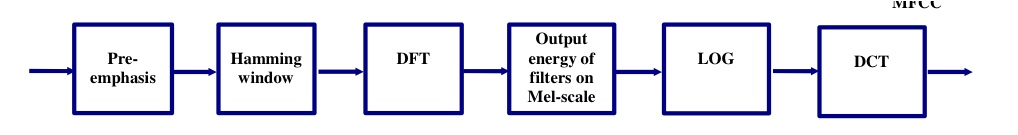
\includegraphics[scale=0.8]{mfcc.jpg}
  \caption{MFCC feature extraction}
  \end{figure}
\begin{enumerate}[label=\roman*]
\item Pre-emphasis: boosts the energy of the signal at high frequencies to improve phone detection
\item Windowing: partitions the time series sequence into frames using a hamming window
\item DFT: extracts spectral information at different frequency bands
\item Mel scale : transforming to mel scale improves recognition performance by allowing the model to take into account the property of human hearing
\item Log : makes the feature less sensitive to variations in input such as power variations on the speakers mouth.
\item Cepstrum : separate the information of the vocal tract from the glottal source. The first 12 cepstral values from spectrum of the log of the spectrum  are used
\end{enumerate}

The windowing process  reduces the length of the time-series sequences. Each sequence is segmented into frames of length 20 to 30 ms. The individual frames are then mapped using the procedure above to MFCC feature vectors where each MFCC vector is extracted from a particular frame. These feature vectors capture information about the positions of the vocal tract of speakers which as I have stated  above is a key attribute in identifying phones. Since the result sequence of vectors is much smaller than the length of the original sequence, the size of the DTW cost matrix is much smaller than before which in turn lowers the time and computation cost incurred by the algorithm. The time complexity of DTW is now reduced from O($n^2$) to O ($u^2$) where $u= \frac{n}{l} $ (l denotes the length of the frame. 

The experiments conducted in section 4.1.1 and 4.1.2, have shown that the  DTW algorithm performs very poorly in terms of accuracy on the TIDIGITS test data when it employs the narrow Sakoe-Chuba band to minimise  the time complexity. The reason for this low accuracy was credited to the influence of  one or  a combination of the following factors : using a narrow window constraint, using raw attribute values and not using domain-dependent features. Having already investigated the influence of using raw values(4.1), for this part of the project, I constructed the  following 3 methods in order to investigate the relative isolated impacts of the other two factors. The methods were  tested on the TIDIGITS dataset, thus allowing the results to be compared with the results of the previous experiments so far :
\begin{enumerate}[label=\roman{*}]
\item The first method  denoted as \textbf{M3} employs the  MFCC feature extraction mapping as a preprocessing step. The extracted features are used  by the valued-based DTW algorithm augmented with the adaptive Sakoe-Chuba band constraint described in 4.1.1 to cluster similar patterns. The performance of this method can be compared to the  performance of the base line method \textbf{M0}  to measure the relative impact  on the accuracy and run-time of the DTW  of replacing each numerical value associated with  each time index with a domain dependent feature vector.
 \item The second method denoted as \textbf{M4} employs a two stage preprocessing step. The feature selection procedure  discussed in 4.1.1  is first applied to remove redundant features followed by MFCC feature extraction that achieves further dimensionality reduction. In this methodology, dimensionality reduction occurs at both stages of the pre-processing step. The downsampling method discussed in 4.1.2  was deemed not necessary as a  feature selection step since the feature extraction phase allows further reduction in dimensionality without any loss of information. The sequence of vectors are then used by the  DTW  algorithm to find optimal warping along the main diagonal of the DTW cost matrix. 
 
 By comparing the results of this method with the results of  \textbf{M3} and \textbf{M1}, the optimum preprocessing strategy can be determined.
\item  The third method denoted as \textbf{M5} is identical to \textbf{M4} with the exception that this version does not employ the window constraint. 
The main purpose of using this method is to check the relative impact  of using window constraints. The difference in the performance between using method \textbf{M4} and \textbf{M5} can be used to check to what degree is employing such a rigid window constraint affects the accuracy and run-time of the algorithm. 

The reason why I opted not to compare the performance of the classifier when it uses  the baseline DTW algorithm(Chapter 3) with raw features against when it employs the window constrained DTW(discussed in 4.1.1) with raw features is that this particular dataset contains  `raw' sequences whose average length is about 7000. If no window constraint is applied, the run time incurred by the 1NN classifier using the baseline DTW algorithm on the `raw' sequences  will be very high. Thus to investigate the improvement in the accuracy of the DTW algorithm, without being disadvantaged with high run times, I have compared the accuracies of 1NN classifier when it employs method \textbf{M4} and when it employs method \textbf{M5} instead. 

\end{enumerate}
Experimental setup:

  \textbf{Dataset} : The TIDIGITS  training and test set (Chapter 2, 4.1.1)
  
\textbf{RESULTS}:



\begin{figure}[H]
  \centering
   
     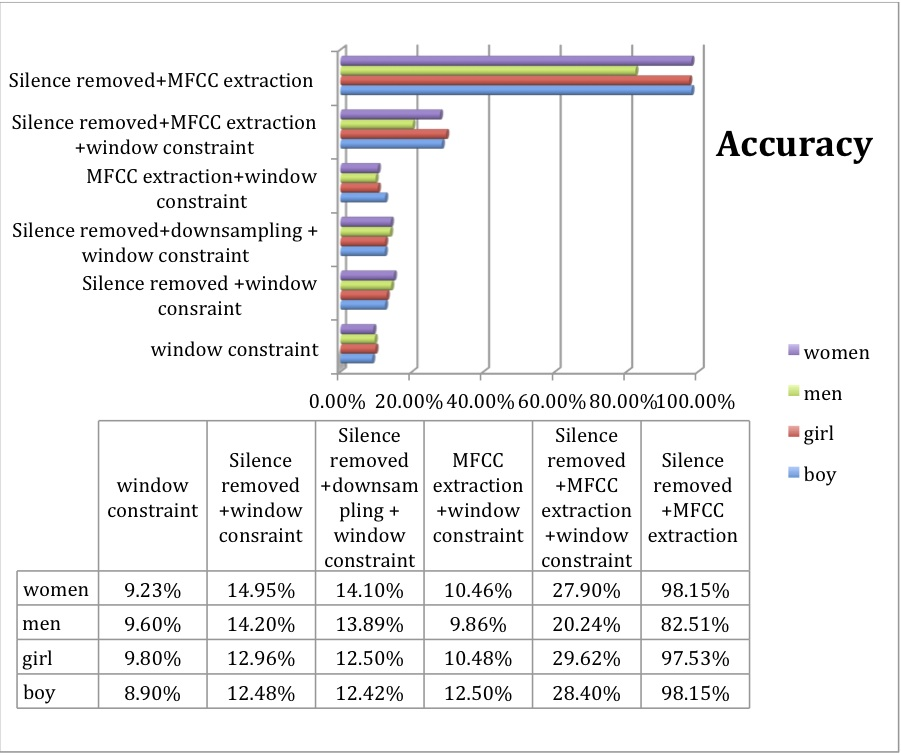
\includegraphics[scale=0.7]{421.jpg}
  \caption{Accuracy achieved by combining 1NN classifier using the DTW distance metrics with the various methods}
  \end{figure}
  
\begin{figure}[H]
  \centering
   
     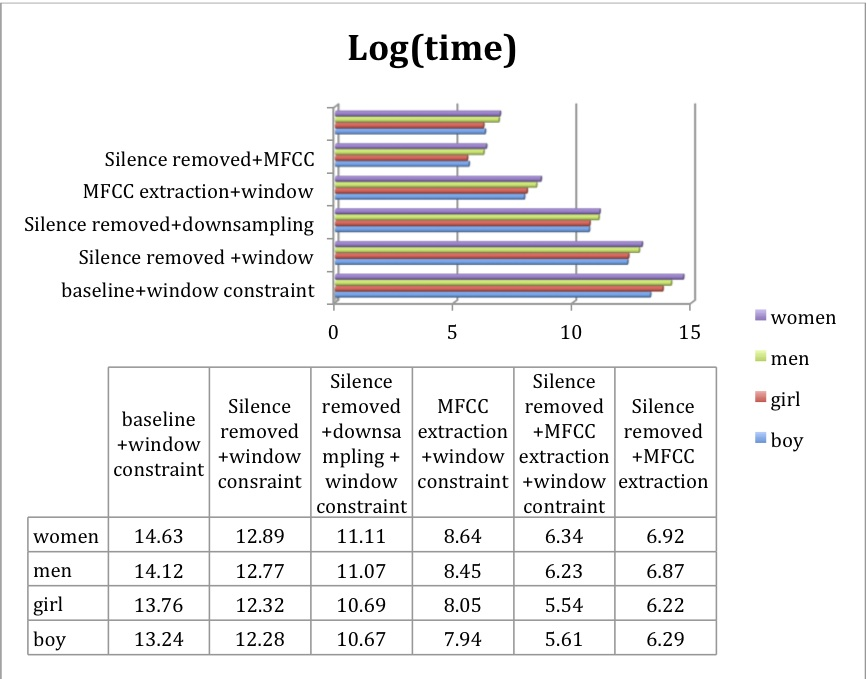
\includegraphics[scale=0.7]{422.jpg}
  \caption{The ln of the run time(measured in seconds) incurred by the 1NN classiier}
  \end{figure}

  Observations:

  
  \begin{itemize}
 \item By comparing the baseline method \textbf{M0} with method \textbf{M3}, we can observe that making DTW domain-dependent has little significance on the accuracy when constraints are employed to minimise the time complexity.
 
 -In comparison to the base-line method \textbf{M0}, the accuracy of the window-constrained DTW  only increases by 1.3\% on average  across all 4 categories. 
 
 -The run-time on the other hand has improved considerably. The average ln(run time) has decreased by 5.7. This is obvious since the acoustic signal is mapped to smaller sequence of frames.  
 
  \item Removing redundant features have greater relative impact on the accuracy than employing domain dependent MFCC features. This is evident  if we compare the accuracy of the 1NN classifier  when it uses the  method \textbf{M2} against the accuracy achieved when it uses  method \textbf{M3}. The presence of silence regions force the optimal warping paths between  patterns of the same lexical identity to lie outside the regions in the cost matrix bounded by the Sakoe-Chuba band. This forces the DTW to find an \textbf{approximate} optimal path with in the allowed regions which in turn leads to an increase in the error rate.
 
   \item Combining  attribute/feature selection with MFCC feature extraction as a preprocessing step (i.e methods \textbf{M4} and \textbf{M5} ) achieves greater improvement in accuracy and speed than using either of these approaches alone. 
   
 -In comparison to just using MFCC feature extraction as a preprocessing step( method \textbf{M3}), the accuracy has been boosted up by 15.17\% on average  while the $ln(time)$ have been reduced by 2.36.  
   
-- Similarly, in comparison  to just using  silence removal as a preprocessing step i.e method \textbf{M1}, the accuracy has  increased  by 12.9\% on average  while the $ln(time)$ have been reduced by 6.5.
  \item  From the above observation alone, we can deduce two facts for this dataset, one of which is not that obvious: removing redundant features have a greater relative impact  on improving the performance of a constrained DTW than employing domain dependent features and the second fact which is quite obvious is the strong dependency between the algorithm's accuracy and the size of the window constraint. It can be concluded that  the use of the rigid window constraint is the main contributing factor for achieving small accuracy rates.
 
Since the main goal is to improve  \textbf{both} the accuracy and  speed of DTW in handling sequences of high-dimensionality i.e long lengths, removal of silence segments provides an ideal mechanism to improve  \textbf{both}  the time complexity and the accuracy of the algorithm. Dropping the window constraint on the other hand, will although lead to considerable increase in the accuracy by will result longer run-times. This is not ideal when working on large high dimensional datasets.
  
  \item Employing Method \textbf{M5} achieves almost near perfect accuracy. Dropping the window constraint of the DTW improves the accuracy of the 1NN classifier by 67.15\% from the accuracy achieved by the classifier when it employs method \textbf{M4}.  In other words 67.15\% of the  time on average, the optimum warping path lie outside the regions bounded by the Sakoe-Chuba band constraints, This confirms  that  patterns belonging to the same lexical identity can have an \emph{overly temporal askew} between them as result of the different contexts in which the words are spoken and/or as a result of different speakers speaking the same word.
  
 \item The run time incurred by the 1NN classifier using method \textbf{M5} is lower than the run time of  all proposed methods with the exception of using method \textbf{M4}. Method \textbf{M5} therefore provides the best balance in the fulfilling  the two  conflicting objectives  of high accuracy and high speed  that any of the other investigated methods.
 \end{itemize}

\textbf{ Conclusion}

To summarise, to improve the performance of the DTW algorithm:
\begin{itemize}
\item In 4.1, I have investigated ways to remove redundant features by conducting exploratory data analysis.

\item In 4.2, I introduced domain dependent feature extraction methods and investigated the influence of the use of such features on the performance of DTW

\item I have investigated the  investigated the relative isolated impacts of using raw values, employing a rigid window constraint and using domain dependent features on the performance of the DTW algorithm

\item I have observed that although the DTW algorithm is domain independent,  augmenting the DTW with a  domain dependent preprocessing technique can greatly improve its performance in terms of \textbf{both} accuracy and speed with out the need of any global constraints.  For the TIDIGITS dataset, employing the preprocessing steps of `silence' removal followed by MFCC feature extraction allows DTW to improve not only its accuracy but also speed  even without the use of global window constraints.
\end{itemize}


 \include{chap4}
 \chapter{Domain Independent methods for Improving DTW}
 
So far, we have investigated methodologies  that  improve both the speed and accuracy of the DTW algorithm by integrating meta data (i.e knowledge of the domain) in the preprocessing stage. The problem with such methodologies is that  the same algorithm cannot be extended across multiple domains: the MFCC feature extraction discussed in the previous chapter is only applicable to time series sequences that correspond to speech utterances. To develop a framework that can be extended across multiple domains, it is necessary to use features that are entirely data driven. In the first half of this chapter, I investigate in detail a  recently proposed data driven feature extraction methodology \citep{Xie2010} that is aimed to improve the accuracy of the DTW across multiple domains. In the second half of this chapter, I investigate alternative measures to using window constraints that can improve the performance of the  algorithm in  terms of \textbf{both} time and accuracy across different  time series domains.

 \section{ Domain-independent feature extraction}

Ideally, we require features that reflect information about the structure of the data. This allows the DTW to construct a complete `picture' of the data point by capturing its relation to the rest of the sequence. Thus, by doing so we can achieve  optimal alignments that are close to the diagonal  for similar sequences. The fundamental problem of baseline (value-based) DTW  is that the  `raw' numerical value associated with each point in the  time series sequence is not a complete picture of the data point  in relation to the rest of the sequence. The context such as the position of the points in relation to their neighbours is ignored. To fix  this issue, an alternative  form of DTW known as \emph{derivative} DTW\citep{Keogh2001} is proposed but  it  too fails to achieve better performance across all domains as it ignores to take into account the common sub-patterns between two sequences (mainly global trends). 

To address these drawbacks, recent works have been conducted to construct good feature extraction methods that are entirely data-driven. One particular approach that has been seen to achieve good accuracies across multiple domains is  the method proposed  by Xie and Wiltgen in their  paper \citep{Xie2010}. The authors highlight a domain-independent feature extraction process where each point in the time series sequence is replaced by a 4 dimensional vector. This 4-d vector attempts to provide a complete picture of a point in  the relation to the rest of the sequence. The  first two features in this vector hold information of the local trends around a point while the last two features reflect information about the global trends. From experiments conducted on the UCR datasets,  they have observed that embedding DTW with this feature extraction process yields greater accuracy across all datasets. 

Definition of local feature given in \citep{Xie2010} is as follows:
\[ f_{\mbox{local}}(t_i)= (y_i-y_{i-1}, y_i-y_{i+1})\]
The first feature reflects the difference between the  values of the current index and the previous index while the second feature corresponds to the difference between the value of the current index and the succeeding index.

The  extraction of global features however, is constrained by two factors:
\begin{spacing}{1}
\begin{itemize}
\item the features must reflect information about  global trends 
\item the features must be in the same scaling order  as the local features. Being in the same scale allows them to  be combined with local features. 
\end{itemize}
\end{spacing}
In \citep{Xie2010}, the authors used the following method to extract global features from the time series sequence:
\[ f_{\mbox{global}}(t_i)= (y_i -\sum_{k=1}^{i-1}\frac{y_k}{i-1} , y_i-\sum_{k=i+1}^M \frac{y_k}{M-i})\]
The first  feature represents the deviation of the value at time i from the mean of the values of the sequence that has  been seen so far while the second feature represents the  deviation  of the value at time i from the mean of the values that is yet to be seen. This formulation allows the detection of significant `drops' or `rises' in the series.


\textbf{Note} : The local and global features have no definition for the first and last points in a sequence and to keep the terminology clear, when I refer to the dimension of the time series, I mean the length of the time series. 

One of the drawbacks of using this feature extraction methodology is the absence of achieving dimensionality reduction. The length of the sequence of vectors is approximately the same as the dimensionality of the original sequence. The DTW algorithm combined with this feature extraction process therefore suffers from the curse of dimensionality as before. Since minimising the time complexity is a major priority for this analysis, the DTW algorithm is subjected to the adaptive Sakoe-Chuba band window constraint discussed in 4.1.1 to minimise the run time.

Xie and Witgen \citep{Xie2010} have already shown that  augmenting this feature extraction methodology to the DTW algorithm improves its accuracy across different domains. However, in their analysis due to the availability of sufficient computing power, they didn't use any window constraints when performing their experiments. For problem scenarios where availability of computing power is limited and  the speed of the DTW is considered an equal priority along with the accuracy, it will be interesting to investigate whether this methodology can allow DTW to achieve better performance in terms of accuracy over  the base line method.
 
To investigate the effect of introducing this prior feature selection step,  I conducted the following 2 experiments:

\textbf{Objective}
Compare the affect between using global and local features and using raw values on the performance of the 1 NN classifier employing a \textbf{window constrained} DTW algorithm.

\begin{itemize}
\item   Experiment 1

\textbf{Datasets}: TIDIGITS dataset(4.1.1)

\textbf{Setup}
Prior to extracting these domain independent features, I performed the feature selection step (\textbf{M1}) which involves removing segments of utterances that correspond to silence. When conducting experiments using MFCC feature vectors, removing redundancy allows the optimal warping paths between similar patterns to lie closer to the main diagonal. Using this feature selection step also has the advantage of dimensionality reduction.

 By comparing the experimental results of this proposed method, which I denote as method \textbf{M6} for simplicity purposes,  with the baseline method \textbf{M0} and method \textbf{M1}, we can observe whether for the TIDIGITS dataset, removing redundant features is more significant to using features that capture information about the global and local trends. Plus, this will allows us  to investigate whether using such features allow a constrained DTW algorithm to achieve higher accuracies  than using raw values.

  

\textbf{RESULTS}

A summary of the results are given below:
\begin{figure}[H]
  \centering
      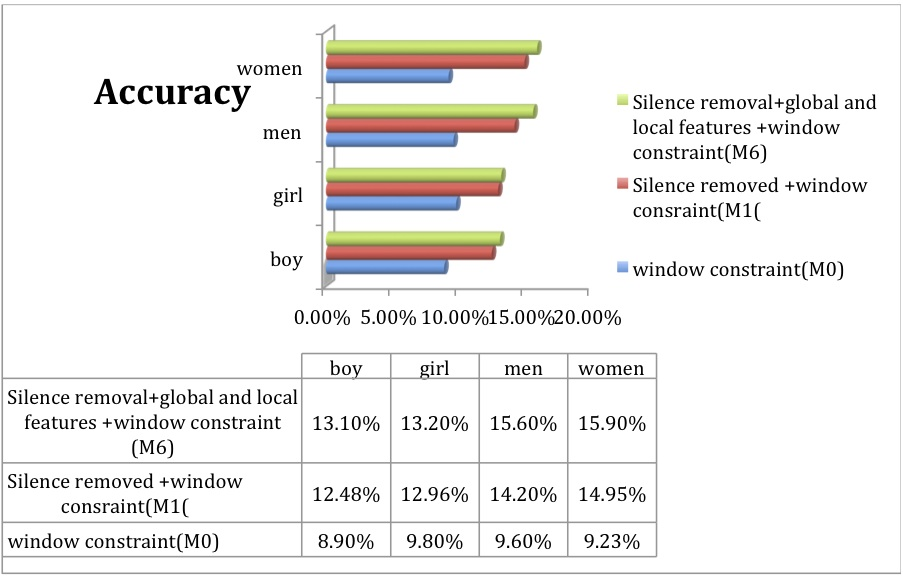
\includegraphics[scale=0.7]{425.jpg}
  \caption{}
  \end{figure}
\begin{figure}[H]
  \centering
     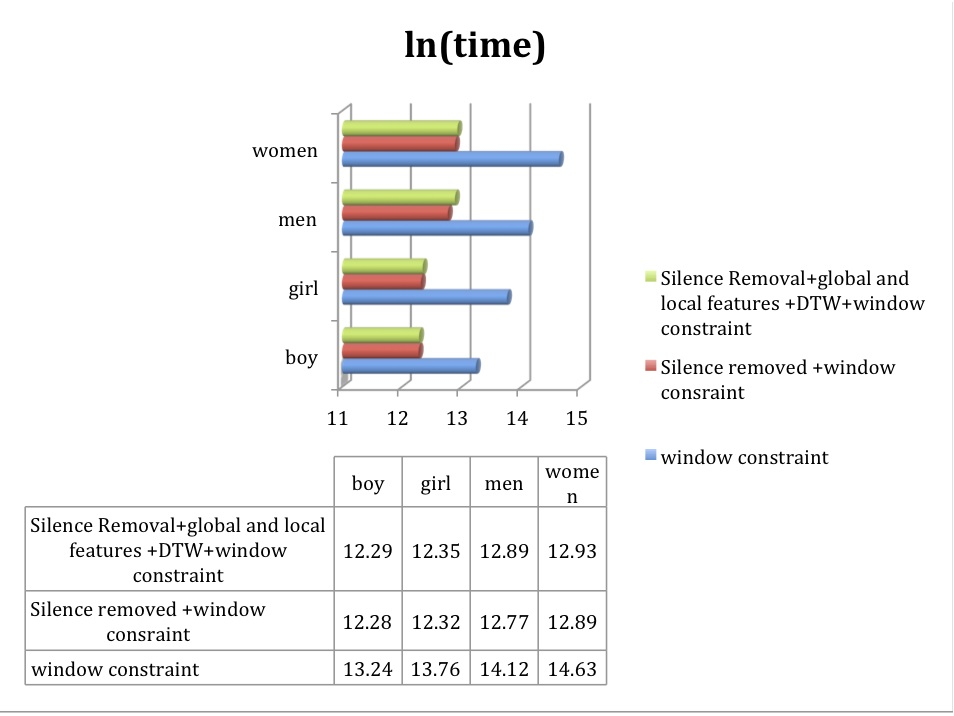
\includegraphics[scale=0.7]{426.jpg}
  \caption{ln of the run time(measured in seconds): $log_e(time)$}
  
\end{figure}
\textbf{Observations}:
\begin{itemize}
\item Removing redundant features i.e  removing regions of silence  is a greater contributing factor in improving the performance of a window constrained DTW than applying a feature extraction process that integrates meta data(\textbf{M3})  or that captures information about local and global trends(\textbf{M6}).  
\item The 1NN classifier combined with the DTW algorithm  achieves very low accuracies  for all 3 methods. As concluded from previous experiments, the low accuracy is primarily credited to the use of the rigid window constraint.
\item  
The computational cost incurred by the 1NN classifier using method \textbf{M6} is higher than when it uses method \textbf{M1}. One possible explanation is that the cost of applying the euclidean metric on vectors $> $cost of applying the euclidean metric on points. Since the euclidean metric is applied $mn$ times where \emph{m} and \emph{n} represent the length of the respective sequences, the  overall computational cost therefore increases.


\end{itemize}




\item Experiment 2

\textbf{Datasets}: UCR datasets: InlineSkate and Cinc\_ECG\_Torso
\end{itemize}
The results are as follows:
\begin{figure}[H]
  \centering
   
     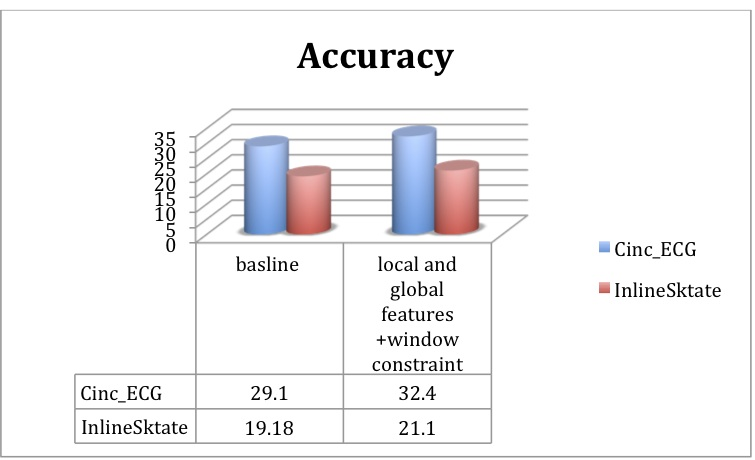
\includegraphics[scale=0.7]{427.jpg}
  \caption{Using features that reflect information of trends improves the accuracy of the algorithm}
  \end{figure}
\begin{figure}[H]
  \centering
   
     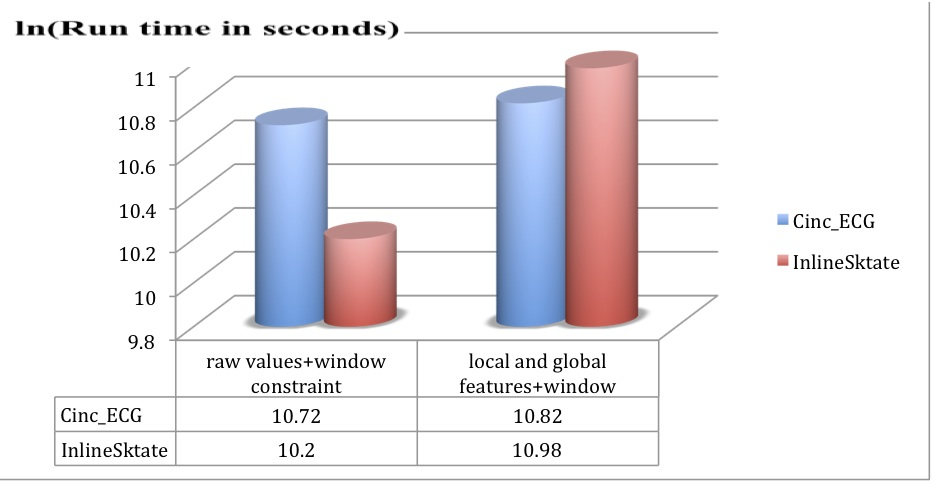
\includegraphics[scale=0.7]{428.jpg}
  \caption{ln of the run time(measured in seconds): $log_e(time)$ }
  \end{figure}
 
 \textbf{Observations} 
  \begin{itemize}
\item The differences between performances of  the two versions of DTW are consistent  with the observations made in the previous experiment. 
\item In comparison to the base line method, there is only a minimum improvement in the accuracy of the window constrained DTW.  For the Cinc\_ECG\_Torso  time series dataset, using global and local features improves the accuracy by only 3.2\%  whereas  for the InlineSkate dataset, the accuracy improves by only 1.92\%.
  \end{itemize}

\textbf{Conclusion}:

 The experiments conducted by Xie and Witgen\citep{Xie2010} on the UCR datasets have shown that using their feature extraction methodology allow DTW to achieve much higher accuracies than using just `raw' values . Optimal paths that closer to the diagonal region of the cost matrix have smaller distances than paths that are further away from the diagonal. The improved accuracy is credited to the construction of optimal paths that are closer to the diagonal than before for sequences belonging to the same class. However the results from their experiments do not provide any information on the degree of translation undergone by these warping paths. The results from my experiments provides this \textbf{insight}. Using the domain independent methodology only leads to a fractional increase in the accuracy of the DTW when it employs a window constraint. This shows that for similar patterns, the degree of translation undergone by the optimal warping paths is very small since very few ideal optimal paths enter the region defined by  Sakoe-Chuba band.
 
  
 The low accuracies of the DTW can be improved by increasing the width of the Sakoe-Chuba band. But increasing the width also leads  to a  reduction in speed. This provides the motivation to investigate alternative methods that can a better balance between the two conflicting goals of accuracy and speed. 
In the next section, I investigate a self-proposed method that is  an alternative approach to using window constraints to speed up DTW. The new proposed methodology uses the data-driven feature extraction process that is discussed in the current section. The aim here to construct a domain independent framework that allows DTW to attain improvements in both speed and accuracy over the  Sakoe-Chuba band window constrained DTW.
 


\section{Extending  DTW}
The feature extraction methodology discussed  in the previous section  offers no advantage of dimensionality reduction. The time series sequence  is mapped to sequence of vectors whose length  is $\|X_n\|-2. $   ( where $\|X_n\| $ denotes the  length of the original time series sequence).  The MFCC feature extraction process (4.2)  on the other hand, does provide the advantage of dimensionality reduction. The time series sequence is first segmented into series of frames  of length 20ms i.e 200 points. Through appropriate functional mapping, each  frame is then mapped to a vector. Hence the time complexity of the DTW algorithm have been reduced from O($n^2$) to  O ($u^2$) where $u= \frac{n}{l} $ ( l denotes the length of the frame). 


Using the MFCC feature extraction method as motivation, I propose the following methodology:
\begin{enumerate}[label=\roman*]
\item Apply the feature extraction process of 5.1 to embed the information of local and global trends.
\item Partition the sequence of vectors into frames of width $m$. The default value of $m$ is set to 50.  Results from experiment 3 discussed later in the chapter have shown that choosing  the default value  to be 50 is a safe option in improving the DTW algorithm's accuracy and speed. For speech utterances in the TIDIGITS dataset, this is equivalent to having frames of size 5ms.  Unlike the windowing process of MFCC extraction, the frames here correspond to sequence of vectors rather sequence of numerical values. This partitioning process reduces the length of the sequences by $m$ times and hence decreases the time complexity of the DTW algorithm from O($n^2$) to O${(\frac{n}{m})}^2$.
\item Adapt the cost metric of the DTW algorithm to work on series of frames  rather than series of vectors 
\end{enumerate}

The problem can now be shifted to finding  an appropriate kernel that can be used to compute the similarity between frames composed of feature vectors. Ideally, we want a metric that takes into account the variation of speed and time when comparing two similar subsequences. To understand why we need the metric to be invariant to variations in speed and time, lets consider the following two signals:

%.  
\begin{figure}[H]
  \centering
   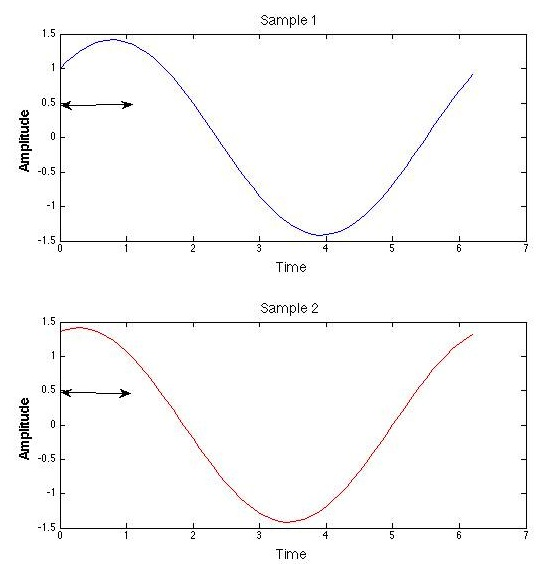
\includegraphics[scale=0.3]{Example1.jpg}
  \caption{Two signals separated by translation}
 \end{figure}
The signal denoted by the `red' color is a `slower' version of the signal denoted by the `blue' color. Consider the frames  corresponding to the subsequences annotated by the double arrows(see figure 5.5), in each of the two signals, in this scenario  using  the Euclidean metric to perform a linear comparison of the two frames is inappropriate. The Euclidean metric  in this context is identical to  linear time warping where the  two subsequences/frames will be compared based on a linear match of the  temporal dimensions of the two sequences/frames.  In our context, we need a kernel that computes the similarity between two sub-sequences by warping the time axis. Intuitively speaking, the kernel must behave like a DTW algorithm that compares the global and local properties associated with a point in one frame with the global and local properties of all points in the second frame as illustrated by the figure below.\\
\begin{figure}[H]
  \centering
   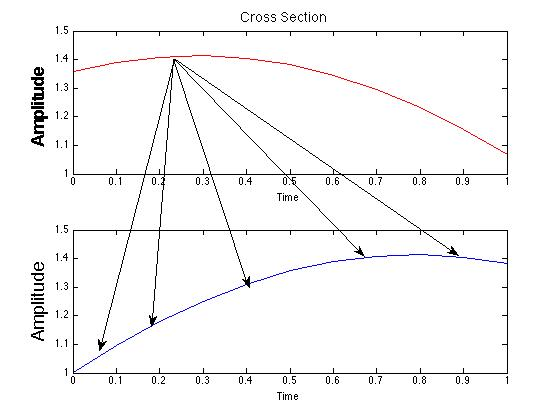
\includegraphics[scale=0.4]{Cross-section.jpg}
  \caption{Two identical subsequences varying in time }
  \end{figure}

The motivation behind my proposed kernel function comes from the polynomial kernel. 
Let $x$ and $z$ be two two-dimensional vectors and consider the simple polynomial kernel of degree 2  :$k(x,z) = (x^{T}z)^2$ .  This kernel can expressed as :
\begin{eqnarray*}
k(x,z) &= &(x^{T}x')^2\\
&  =& (x_1z_1+x_2z_2)^2\\
&= & x_1^2z_1^2 + 2x_1z_1x_2z_2 + x_2^2z_2^2\\ 
&=& (x_1^2, �2x_1x_2, x_2^2)(z_1^2, �2z_1z_2, z_2^2)^{T}\\
&=& \phi(x)^{T}\phi(z)\\
\end{eqnarray*}\\
The 2nd order polynomial kernel is equivalent to a corresponding feature mapping $\phi(x)$  that  maps a two dimensional vector to $(x_1^2, �2x_1x_2, x_2^2)$ where each attribute is monomial of order 2 . Generalising this notion to order M then $k(x,z) = (x^{T}z)^M$ represents the sum of all monomials of order M. If we imagine x and z to be two images, then the polynomial kernel represents a particular \textbf{weighted} sum of all possible products of M pixels in the first image with M pixels in the second image.\\
Using this as motivation I propose the following kernel:.
\[ k(x,z) = <\sum_{i=1}^{n}x_i, \sum_{j=1}^{n}z_j>\]
Here $n$ denotes the length of the frame while $x_i$  and $z_j$ correspond to the individual 4-dimensional feature vectors that make up  the frame. The above kernel corresponds to the dot product between  the individual sums of the two frames. Although it may not look obvious, this construction actually allows the comparison between all feature vectors in the first frame with all feature vectors in the second frame as shown below:
\begin{eqnarray*}
k(x,z) &= &<\sum_{i=1}^{n}x_i, \sum_{j=1}^{n}z_i>\\
&  =& <(x_1+x_2+x_3+..),(z_1+z_2+z_3+..)>\\
&= & <x_1,z_1>+<x_1,z_2>+<x_1,z_2>...+<x_2,z_1>+<x_2,z_2> +...
\end{eqnarray*}
From above expression, we can see  that the proposed kernel corresponds to a sum of all possible dot products of pairs belonging to the set
$\{(x_iz_i) | x_i\in \mbox{seq1}, z_i \in \mbox{seq2}\}$. It is easy to check that this proposed kernel is in fact a valid kernel function:
\begin{itemize} \itemsep-2pt
\item K(x,z)= K(z,x) $\Rightarrow $the function is symmetric.
\item The kernel can be written as a scalar product in feature space: K(x,z) =$\phi(x)^T\phi(x)$
where  the feature mapping corresponds to  a finite summation of vectors $\phi(y) = \sum_{i=1}^{n}y_i$. 
\end{itemize}

Augmenting the kernel to the DTW algorithm allows DTW to work on long time sequences without using a window constraint.
%\begin{itemize} \itemsep-2pt
%\item The accuracy of DTW increases as the width of the windows decrease. Using subsequence allows the similarity measure to be dominated by the dot products of points whose local and global features are most alike. However using smaller windows achieve lesser dimensionality reduction. Thus the time and computational complexity suffers.
%\end{itemize}
To use this kernel as an  appropriate cost function in the DTW algorithm, we need a functional mapping that:
\begin{enumerate} \itemsep-2pt
\item  constraints the codomain to be in the range from 0 to $\infty$.
\item    ensures larger values given by the function signify great degree of dissimilarity and smaller values  signify a high degree of similitude.
\end{enumerate}
An inspection of the kernel function shows the function represents the sum of dot products of all vectors in one frame with all vectors in the second frame. An  ideal cost function that make use of dot products is the \emph{arc-cosine}. Using an appropriate substitution, I have thus constructed the following cost metric:  
\[ \theta = \frac{ <X,Z>}{|X||Z|} \]
where $\theta$ is the \emph{arc-cosine} distance, $X = \sum_{i=1}^{n}x_i$ and $Z =\sum_{j=1}^{n}z_i$.

A formal outline of the proposed methodology is  given by the following algorithm:

 \begin{algorithm}[H]
\begin{algorithmic}
\Procedure{Value-based}{$seq1,seq2$}\Comment{two sequences of feature vectors}
\State  seq\_1$\leftarrow$segment(seq1,n)\Comment{ Segment the sequences using a window of size n}
 \State seq\_2$\leftarrow$segment(seq2,n)
 \For{i=1: to length(seq\_1) } \Comment{Initialise the DTW cost matrix}
 \State DTW(i,0) = $\infty$
 \EndFor
 
 \For{i=1 to length(seq\_2)}
 \State DTW(0,i) = $\infty$
 \EndFor
  \For{i=2 to length(seq\_1)}  
 \For{j=max(2, i-w) to min(length(seq\_2), i+w)} 
 
  \State DTW(i,j) = $\theta = \frac{ <X,Z>}{|X||Z|} $+ min\{ DTW(i-1,j)+DTW(i,j-1)+DTW(i-1,j-1)\}
 \EndFor \Comment { $X = \sum_{i=1}^{n}x_i$ and $Z =\sum_{j=1}^{n}z_i$}

 
 \EndFor
\State \textbf{return}  result = $\frac{\mbox{DTW(n,m)}}{nm}$ \Comment{n=length(seq1), m=length(seq2)}

\EndProcedure
\end{algorithmic}
\caption{Proposed DTW}
\end{algorithm}
 


\subsection{Testing the methodology}
The primary objective is  to improve the performance of the DTW algorithm in problem domains where minimising time complexity shares equal priority with improving accuracy.
To investigate whether the proposed changes does provide a better alternative to using the Sakoe-Chuba band window constraint, I have conducted the following experiments:



\textbf{Experiment 1}

\textbf{Dataset used} : The TIDIGITS dataset.

\textbf{Method used} : The  preprocessing method discussed in 5.1 i.e \textbf{M6}: the  framework consists of a two stage preprocessing step that involves feature selection process consisting of `silence' removal  followed  by the domain  independent feature extraction methodology proposed in \citep{Xie2010}

\textbf{Variables being compared}: Sakoe-Chuba band window constraint VS the proposed methodology

RESULTS: 
 \begin{figure}[h!]
  \centering
      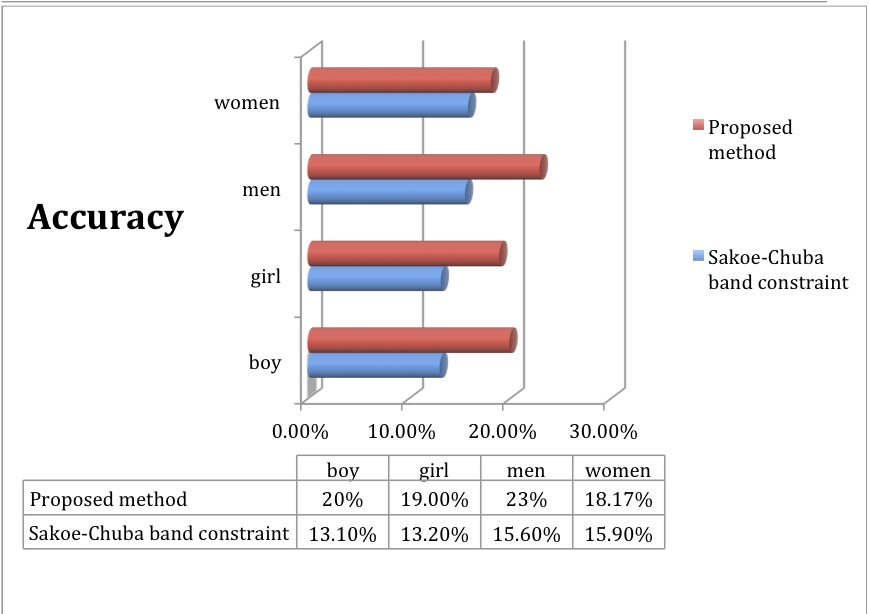
\includegraphics[scale=0.9]{521.jpg}
  \caption{Accuracy}
  \end{figure}

\begin{figure}[H]
  \centering
     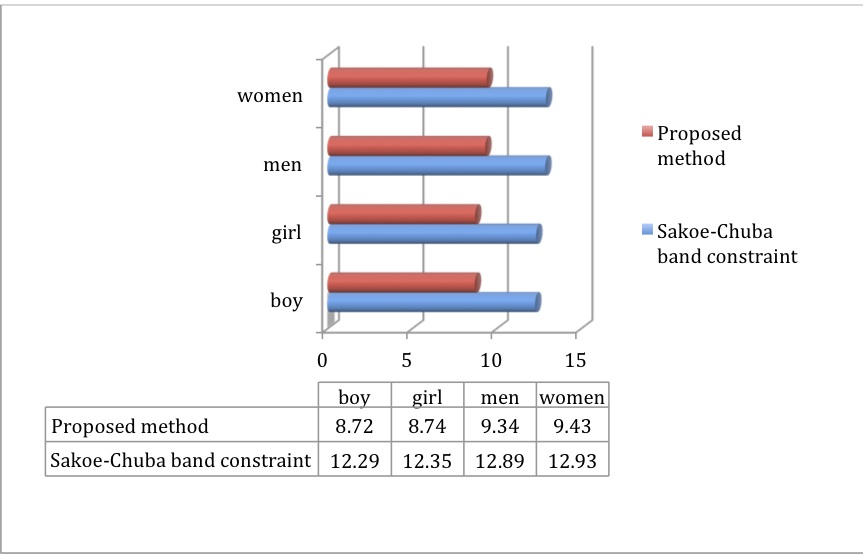
\includegraphics[scale=0.7]{522.jpg}
  \caption{ln of the run time(measured in seconds): $log_e(time)$}
  \end{figure}

There are quite number of interesting observations that can made from  figures 5.7 and 5.8. 

\begin{itemize}
\item In comparison to employing the Sakoe-Chuba band window constraint, the alternative method allows DTW to improve its accuracy across all 4 categories by 6.54\% on average.
\item  Equipped with the new changes, the run time  of the algorithm has decreased exponentially  by an \textbf{order} of 3.1 on average. The reduction of the time complexity is mainly due to the partitioning of the sequence into time slices of width 5 ms.The reduction in the length of the sequences by an order of 50 results in the shrinkage of the search space of DTW thus causing the algorithm to improves its speed.

% In Chapter 3, I have shown that the time complexity of the algorithm  equipped with Sakoe-Chuba band constraint is O(n+wn) where w is the size of the adaptive window. The analysis shows that the time complexity associated with the proposed method is smaller than O(n+wn).

\end{itemize}
%As we have seen so far, increasing the speed of DTW negatively impacts the accuracy of the algorithm . The new methodology actually provides an exception. The use of the kernel function improves the accuracy of the DTW   which implies that matching frames using the new cost function is a better alternative than employing the euclidean distance between points/vectors confined by the window constraint.
The proposed methodology can also be adapted to use domain-dependent features.  As I have stated earlier, the main motivation for constructing this framework is to provide better performance  in terms of both accuracy and run-time for time series problem domains where the use of rigid window constraints is deemed necessary to minimise the computational cost. In the previous chapter, I have discussed that when the MFCC feature extraction is used as the only preprocessing step, the use of the adaptive window constraint was deemed necessary  to minimise the run-time. However from the experimental results in the previous chapter, it was observed that  enforcing such a rigid constraint results in a high error rate. To verify that the new proposed changes  to the  DTW algorithm allow it to perform equally well when using domain dependent features,   I have repeated the same experiment again but this time, as  a preprocessing step  I have  just used  the MFCC feature extraction i.e method \textbf{M3}. 




A summary of the results are as follows:

\textbf{Experiment 2}

\textbf{Dataset used} : The TIDIGITS test and training data.

\textbf{Method} :  \textbf{M3} which consists of single preprocessing step that involves the extraction  of MFCC features

\textbf{Variables being compared}: employing window constraints vs the  new proposed changes

\textbf{Results}
\begin{figure}[h!]
  \centering
      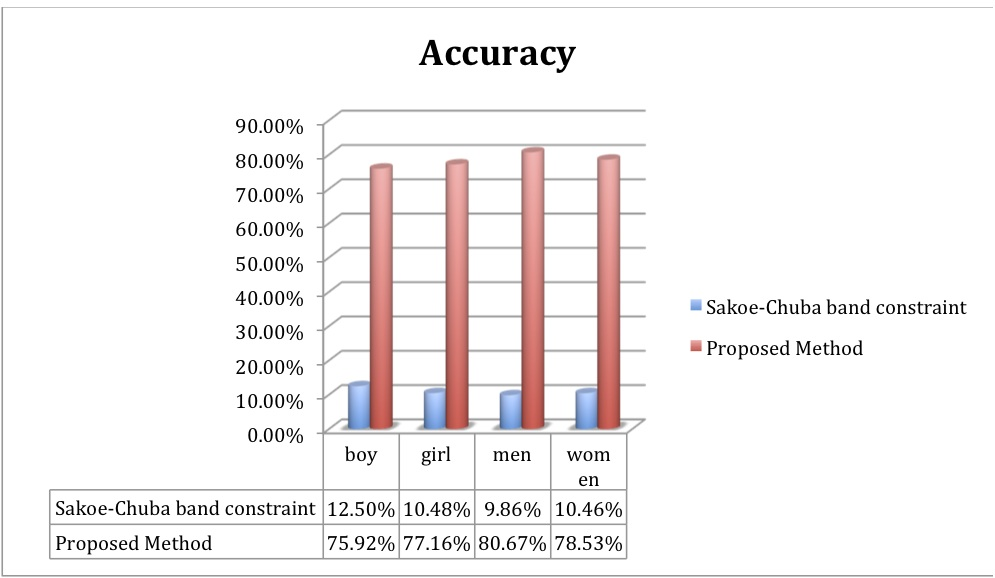
\includegraphics[scale=0.8]{523.jpg}
  \caption{Accuracy}
  \end{figure}

\begin{figure}[H]
  \centering
     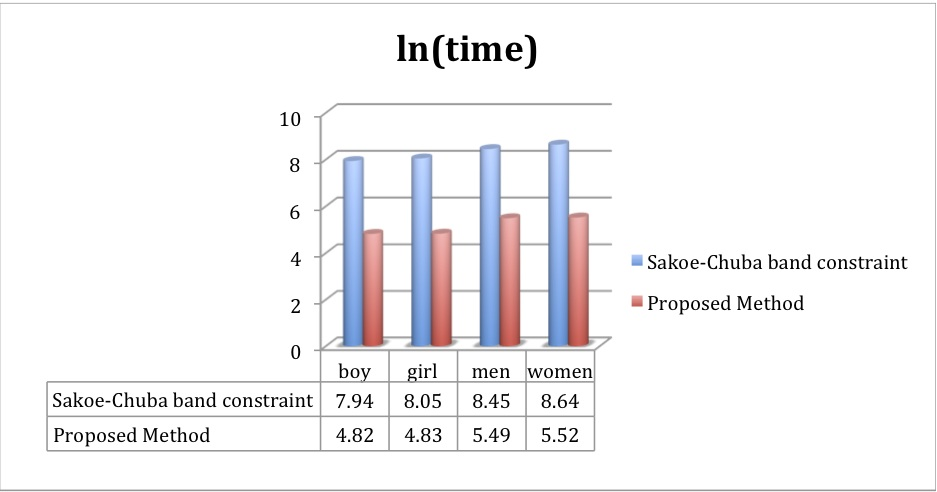
\includegraphics[scale=0.8]{524.jpg}
  \caption{ln of the run time(measured in seconds): $log_e(time)$}
  \end{figure}

\textbf{Observation}
The results are consistent with the findings in the previous experiment. The accuracy of the DTW algorithm has improved by over 60\% on average and the average run time  has decreased exponentially by an order of  3.12. Hence in comparison to the window constrained DTW, the new framework takes better advantage  of employing domain dependent features.

 However, since the tests so far has been conducted on the TIDIGITS test set, it is possible that this new approach is only tailored for this particular dataset. Thus to confirm  that the boost in the performance is not tailored for this particular time-series dataset, I have performed classification using the proposed DTW algorithm on the UCR datasets: InlineSkate and CINC\_ECG\_TORSO and compared the performance against the performance achieved by the 1 NN classifier using the baseline DTW metric augmented with Sakoe-Chuba band constraint discussed in 4.1.1.

\textbf{Experiment 3}

\textbf{Datasets used} : InlineSkate and CINC\_ECG\_TORSO

\textbf{Setup} : 

Method used : The  preprocessing method discussed in 5.1 i.e \textbf{M6}: the  framework consists of a two stage preprocessing step that involves feature selection process consisting of `silence' removal  followed  by the domain  independent feature extraction methodology proposed in \citep{Xie2010}.

In the  proposed approach,  the width of the time slices has been kept fixed at a default value of 50 so far. In this experiment, I also investigate the influence of this parameter on the performance of the DTW. Decreasing its value reduces  the size of the time slices which in  principal should increase both accuracy and time-complexity. This is because  the core kernel used by the new algorithm is : 
\[ k(x,z) = <\sum_{i=1}^{n}x_i, \sum_{j=1}^{n}z_j>\]
 where k(x,z) represents the sum of all possible dot-products. Using smaller subsequences allow the similarity measure to be dominated by the dot products of points whose local and global features are most alike. However,  this suffers from the drawback of achieving lesser dimensionality reduction. Thus the time and computational complexity suffers.

\textbf{RESULTS}

\begin{figure}[H]
  \centering
      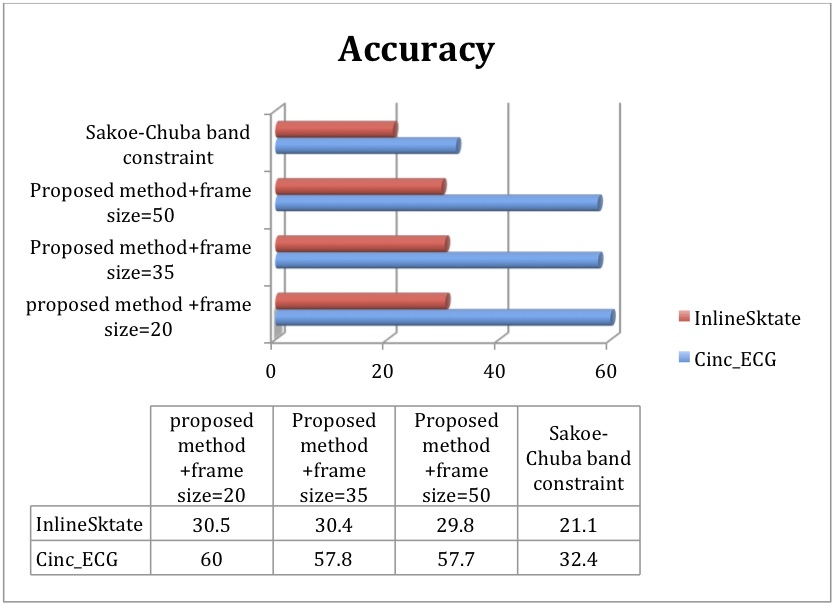
\includegraphics[scale=0.9]{525.jpg}
  \caption{Accuracy}
  \end{figure}

\begin{figure}[H]
  \centering
      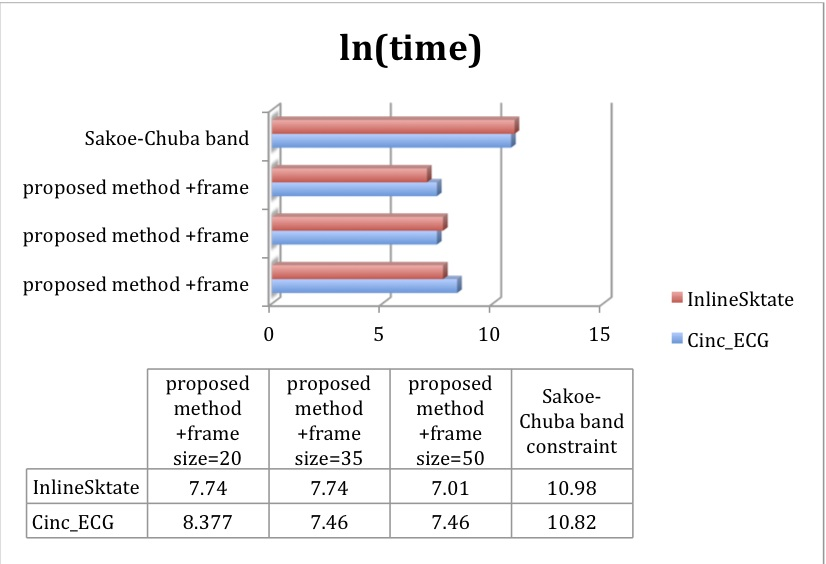
\includegraphics[scale=0.9]{526.jpg}
  \caption{ln of the run time(measured in seconds): $log_e(time)$}
  \end{figure}

\textbf{Observation}

\begin{itemize}
\item The proposed changes do provide  a \textbf{ better} alternative   to using rigid constraints  for problem domains where the time complexity is of high priority and the use of window constraints can not be avoided. The accuracy of the DTW algorithm under the new methodology is significantly higher then employing a window constrained DTW on sequences of extracted local and global feature vectors.  
\item Decreasing the size of the time slices only leads to a minimal increase in accuracy. Thus using the default value of 50  seems to be safe option as the algorithm better accuracy and speed than using the rigid Sakoe-Chuba band constraint .

\end{itemize}
\subsection{Conclusion}

In chapter 3, we have seen that under the window constraint the time complexity of the algorithm decreases from O($n^2$) to O(wn). From the  experimental results, it can be observed that the new proposed changes allow DTW to achieve run times that are exponential lower than the run times achieved by the window constrained DTW. Thus it can be concluded that the  time complexity of the proposed DTW variant is smaller that O(wn). 

 We have seen so far  that increasing the speed of DTW negatively impacts the accuracy of the algorithm . The new methodology actually provides an exception. The use of the kernel function improves the accuracy of the DTW   which implies that matching frames using the new cost function is a better alternative than employing the euclidean distance to find local optimal warp path only through the constraint window.  Combining this approach with the feature extraction method discussed in \citep{Xie2010}  results in the construction of a model  that can applied for \textbf{different types} of time series datasets. 




\include{chap5}
 \chapter{SVD For Time Series Feature Extraction  }
In the previous chapter, we have explored techniques that can improve the performance of the DTW algorithm in handling high dimensional time series sequences. In this and the following chapters, I will be concentrating in improving the accuracy and run-time of the  1NN classifier equipped with the Euclidean metric  on time series sequences. To be precise, I will be exploring feature extraction techniques to extract a smaller set of independent features from the raw sequences that can capture information about the global shape. This formulation will not only achieve dimensionality reduction but  will also allow the time series classification to be treated like a normal classification problem.


\subsection{Motivation}
High dimensional data vectors $\{x_n\}$  typically lie close to a non- linear manifold \citep{bishop2006pattern} whose intrinsic dimensionality is smaller than that of the input space as a result of strong correlations between the input variables. In data mining, to understand this intrinsic dimensionality of the data, the Single Value Decomposition(SVD) algorithm is widely used. SVD  simplifies the data representation by showing only the number of important dimensions that captures the \textbf{variance} of the data. Intuitively speaking, SVD projects the high dimensional data vectors to an orthogonal subspace that maximises the variance of the data. The focus of this chapter is to investigate whether SVD can be applied to time series datasets to extract independent  latent features that  minimise the run time of the 1NN classifier augmented with the euclidean metric.


\section{ Background}

\textbf{The formal definition of SVD as stated in\citep{Marchette1999,Korn1997} is given as follows}:
 
 Any $M \times N $ real matrix  X  can be factorized  of the form $X = U D V ^T$ 
 where 
 \begin{itemize}
 \item  U is a $M \times M $ orthogonal matrix. The columns of U are the eigenvectors of $XX^T$
 \item D is a $M \times N $  rectangular matrix  with :
 \[D_{ij}= 
\begin{cases}
     \sigma^2,& \text{if } j= i\\
    0,              & \text{otherwise} \end{cases}\]
 Here D is a diagonal matrix  where the diagonal entities are called singular values and are  ranked from greatest to least. The number of non-zero singular values determine the rank  of the original matrix. 
 
  \item  V is a $N \times N $ orthogonal matrix. The columns of V are the eigenvectors of $X^TX$. Since $X^TX$ is the covariance matrix, these eigenvectors span the linear subspace that maximises the variance of the data.
 \end{itemize}
 
Dimensionality reduction is achieved by discarding the eigenvectors in V i.e the columns that are associated with the smallest or zero singular values. Thus, each sample can now be represented by fewer dimensions. For data matrices where M $\ll$ N, there exists at most M-1 singular values. In such situations, considering only the non zero columns in the diagonal matrix  D  and the associated columns in V achieves dimensionality reduction without any loss of function.
The data matrix X can be factorized as $X = U\times D'\times V'^T$ where D is now an M by K diagonal matrix containing only positive values on its diagonal and V' is the corresponding N by K matrix. The matrix $V'^TV$ captures the full  covariance of the data. 



 \section{Motivation for applying SVD to  time series datasets}
Unlike other datasets, clustering/classifying time  series sequences by conventional distance metrics, such as the euclidean,  may not result  in high accuracy. The scope of such metrics is quite  limited in the fact that they  require  sequences to share the same length and  comparison of sequences is based on a linear match of the  temporal dimensions of the two sequences. This represents a  substantial drawback as the metrics fail to take into account that similar patterns  may vary in terms of speed, length and scale. Therefore, this provides the motivation to look for  preprocessing feature extraction techniques that can extract translation and scale invariant features that capture information about  the intrinsic trends in the data.

However, recent works have shown that there exists time series domains where the use of conventional methods can still achieve accurate results. Korn in his paper  \citep{Korn1997} has  shown that  for time series sequences that share the same \textbf{speed} and \textbf{length},  the conventional methods can achieve good clustering/classification performance. If  intra class sequences have the same speed i.e no time offsets then they will also share the same time localised trends(see figure 6.1). Applying SVD as a preprocessing step,  results in the  extraction of  latent factors that represent the  localised patterns in time.  Through mapping the time series sequences into the latent space, we can therefore construct a  simplified representation of the data which allows conventional methods such as the euclidean metric to cluster time sequences with lesser run time.

To see how SVD accomplishes this feat, lets consider the following toy example:

 Let  X be  a matrix where rows correspond to customers, columns correspond to days and the values are the dollar amounts spent on phone each day.
 
X = \begin{tabular}{|c|c|c|c|c|c|}
 \hline\\
 customer & wed & thurs & frid & sat & sun \\
 \hline\\
 A & 1 &1 &1 &0 &0 \\
 B  &2& 2& 2& 0& 0 \\
 C &1 &1 &1  &0& 0 \\
 D &5& 5& 5& 0& 0 \\
 E  &0 &0 &0 &2 &2 \\
 F  &0& 0& 0& 3& 3 \\
 G & 0 &0 &0  &1 &1 \\
 \hline
 \end{tabular}

\textbf{Observation}
\begin{itemize}
\item There are only two distinct time localised trends. From this we can infer that there are two groups of customers: one group  makes calls only during week days while the other group makes calls only  during weekends.
\end{itemize}
Using SVD to factorize the matrix gives:

\begin{eqnarray*} 
X & = & U\times D \times V^T\\
 X & = &  \left( \begin{array}{cc}
0.18 & 0 \\
0.36 & 0\\
0.18 & 0 \\
0.90 & 0 \\
0 & 0.53 \\
0 & 0.80 \\
0 & 0.27 \\
\end{array} \right)
\times \left( \begin{array}{cc}
9.64 & 0 \\
0 & 5.29
\end{array} \right)\times
\left( \begin{array}{cc}
0.58 & 0 \\
0.58 & 0 \\
0.58 & 0 \\
0 & 0.71 \\
0 & 0.71 
\end{array} \right)^T\end{eqnarray*}

Note: The columns in the orthogonal matrix V that are the eigenvectors of  the zero singular values in the diagonal matrix have been omitted. Omitting these column vectors results in no loss of information.

\textbf{Key observations}
\begin{itemize}
\item The rank of the matrix X is 2. This shows that there are effectively two groups of customers: weekday(business) and weekend(residential) callers.
\item The U matrix can be thought of as a customer to pattern similarity matrix. The first column vector of U corresponds to the weekday customers while the second column vector represents the weekend customers
\item The V matrix can be thought  of as day to pattern similarity matrix. In the case of days, there are two  patterns: the weekday pattern i.e \{Wed,Thurs,Frid\} and the weekend pattern \{Sat,Sun\}
\end{itemize}

For SVD to be applied successfully across all time series datasets , there are two fundamental issues that must be addressed:
\begin{enumerate}
\item Time complexity: The time complexity of SVD  is O($D^3$) where D represents the dimensionality of the data. For domains where the dimensionality of the data is really high, applying SVD as a preprocessing step increases the run time of a clustering/classification algorithm.


%\item Distortion of time series sequences: Conventional methods  yield poor results in classifying and clustering time series sequences that are distorted by length,scale and speed. This makes methods that combine SVD and 1 nearest neighbours very unattractive to use.
\item Variable  dimensionality:  SVD cannot be directly applied to datasets where the individual data points do not share the same dimensionality. This issue is specially seen in time series data sets such as speech. The acoustics samples in such datasets vary in length.
\end{enumerate}

In the rest of this chapter, I will be focussing on addressing the first issue : the problem of high time complexity that is associated  with  SVD  when handling datasets with long time series sequences.

%To address the above issues and the drawbacks associated with performing nearest neighbours classification on time series sequences, in the following three sections, I investigate :
%\begin{enumerate}[label=\roman{*}]
%\item methods to improve the time complexity of SVD in handling high dimensional sequences when the size of the dataset is very small.
%\%item preprocessing methods that can used along side the SVD feature extraction scheme to boost the accuracy of the classifier  
%\item techniques to adapt SVD in handling  time series sequences of variable length 
%\end{enumerate}


\section {Improving Time Complexity}
 For datasets where N(the number of samples) $\ll$ D(dimensionality of the data), Bishop \citep{bishop2006pattern} offers the following solution that reduces the time complexity of computing SVD from O($D^3$) to O($N^3$):
  
 Let  X  be the constructed  D by N  data matrix where D is the number dimensions and N is the number of samples and  D$\ll$N. By  factorizing X, we get X=$U \times D \times V^T$. To achieve dimensionality reduction, we need to consider only the  subset of  columns vectors of V   that are associated with the non-zero singular values. Since N $\ll$D, there will at most N-1 of these singular values. As stated earlier, the columns of the V are the eigenvectors of the covariance matrix $ XX^T$.
 
 The eigen decomposition of the covariance matrix is $ XX^T u_i= \lambda_i u_i$. $XX^T$ is D by D matrix and the computational complexity of computing the eigenvectors is O ($D^3$).

Now if we multiply both sides by  $X^T$ we get :
\[ (X^T X)X^T u_i = \lambda_i X^T u_i\]
Setting $v_i =X^T u_i$ gives us the eigenvectors of $X^TX$.

From the above expression, it can be observed that the eigenvectors of  $X^TX$ and  $XX^T$ share the \textbf{same} eigenvalues. Using this insight,  we can thus solve the eigenvector problem in spaces of lower dimensionality with computational cost O($N^3$) instead of O($D^3$). The required eigenvectors of the covariance matrix can then be computed by the using the following expression:
\[ u_i = \frac{1} {\lambda^(\frac{1}{2})} Xv_i\]
 
 For each of the time series datasets used in this project, using Bishop's solution, I have extracted  the first k eigenvectors that capture 95\% variation of the data with minimal computation cost. By projecting the time series sequences to the orthogonal subspace spanned by the eigenvectors, I have hence constructed  a compact representation of each time series sequence. This compact representation in turn allows the 1NN classifier to reduce its time complexity from \textbf{O}(ND) to \textbf{O}($N^2$) where N is number the samples,  D is the length of the sequences and $N\ll D$.  
 \subsection{Experimental results}
To verify the above approach,  I have conducted the following experiment :

\textbf{Objective} : The experiment is designed to verify  whether applying SVD as  a preprocessing step can improve the run time of 1 nearest neighbour classifier on time series datasets, without affecting its accuracy.

\textbf{Datasets used} : InLineSkate and Cinc\_ECG\_TORSO. 

Unlike the speech corpus, the time series sequences of each dataset share the same length. This allows metrics such as the euclidean to compare the similarity between two sequences by conducting a linear match of their temporal dimensions. Since the number of samples $\ll$ the length of the sequences, the size of the latent space will be smaller than the original input space. For the UCR datasets, I have considered the first k eigenvectors  of the covariance matrix that capture \textbf{95\%} variation of the data as latent features.

\textbf{Metric Used}: Euclidean distance

\textbf{Methods Compared}: 1NN classifier using SVD as a preprocessing step Vs 1NN classifier
%Unlike the speech corpus, the intra class variance of the time series sequences in the  UCR datasets are much lower. This is primarily due to the fact that sequences of the same class can be described by the same time-localised trends. Figure 6.1 shows examples of two sequences belonging to class `1' in the  Cinc\_ECG\_TORSO dataset. Apart from having the same shape, the two sequences also posses the same speed i.e they have no time offset. From figure 6.1,it can seen that at around t=600, both patterns undergo a dip followed by a sharp peak. The fact that all sequences in the dataset share the same length and intra class sequences have no time offset  allow classification algorithms to treat the problem as a  normal classification problem. This also provide the context to apply SVD  directly to achieve dimensionality reduction. For this experiment, SVD has been applied to extract all the eigenvectors of the covariance matrix that corresponds to non-zero singular values. Since the number of samples $\ll$ the length of the sequences, the size of the latent space will be smaller than the original input space leading to dimensionality reduction without any loss of information. 
%\begin{figure}[H]
  %\centering
    %  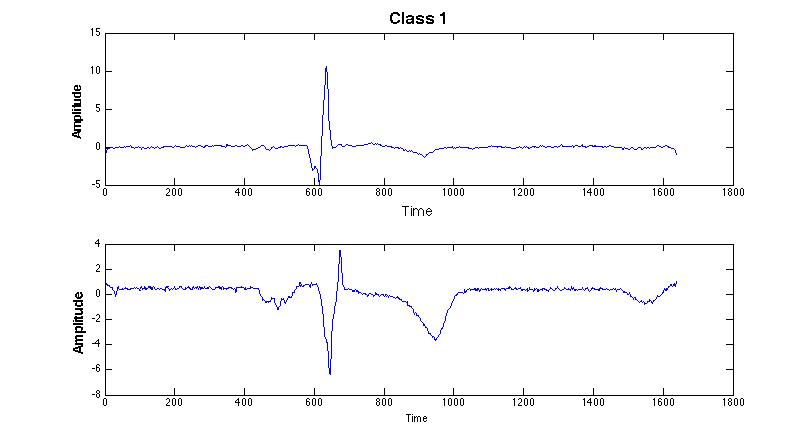
\includegraphics[scale=0.5]{611.jpg}
  %\caption{Time series sequences  corresponding to class `1' in the Cinc\_TORSO\_ECG dataset}
  %\end{figure}

 \textbf{Results}:
\begin{table}[H]
\begin{tabular}{|c|c|c|}
\hline \\
      & SVD+1NN classifier &1NN classiifer \\
      \hline\\
Cinc\_ECG\_TORSO & 89.71 & 89.71 \\
InlineSkate &  34.18 & 34.18 \\
\hline

\end{tabular}
\caption {Accuracy} \label{Accuracy}

\end{table}

 
\begin{table}[H]

\begin{tabular}{|c|c|c|}
\hline \\
      & SVD+1NN classifier &1NN classiifer \\
\hline\\
Cinc\_ECG\_TORSO & 0.77s & 0.88s \\
InlineSkate &  0.48s& 1.03s \\
\hline

\end{tabular}
\caption {Run times in seconds} \label{Run times in seconds}
\end{table}
Note: The time complexity associated with the Euclidean metric is \textbf{O}(N) which is much smaller than \textbf{O}($N^2$) - the time complexity of the DTW algorithm. Thus, the  associated run times associated with the 1NN classifier using the Euclidean metric will be very small in comparison to the run times incurred by the classifier when it employs the DTW metric. Therefore to make effective comparisons of the run times incurred by 1NN classifier equipped with the Euclidean distance  metric for embedding different preprocessing techniques, from now on I will be comparing the run times directly and not the ln of the run times.


\textbf{Observations}

\begin{itemize}
\item The accuracy of the 1 nearest classifier  in both cases is consistent with the  1NN error rate given for each of the datasets  in the UCR data source webpage\citep{UCR}.
\item Applying SVD  as a preprocessing step has no effect on the accuracy on the 1NN classifier but succeeds in reducing the run time of the classifier. Thus using Bishop's\citep{bishop2006pattern} formulation, we can use SVD to reduce the time complexity of clustering/classification algorithms  for high dimensional time series datasets that satisfy the constraints identified by Korn\citep{Korn1997}.
\item 1NN classifier equipped with Euclidean metric achieves very high accuracy for the Cinc\_TORSO\_ECG dataset. The similarity of intra class  sequences  for this dataset can be classified fairly accurately by performing only a linear match of their temporal dimensions. From this observation, we can conclude sequences belonging to the same class   tend to  share the similar \textbf{time localised }i.e time aligned local  and global trends.
\item Using the euclidean metric, the 1 NN classifier is seen to achieve very low accuracy for InlineSkate dataset.This shows that unlike the Cinc\_TORSO\_ECG datasets, the intra class sequences are not aligned with respect to the time axis.

\end{itemize}
%In order to analyze a nonstationary signal, we need to determine its behavior at any individual event. Multiresolution analysis provides one means to do this. A multiresolution analysis decomposes a signal into a smoothed version of the original signal and a set of detail information at different scales. The procedure is recursive. After removing the first set of detail information from f we are left with a slightly smoothed version of f. Iteratively removing detail information progressively generates more andmore smoothed versions of f. We stop the process once we have enough detail information or a smooth enough version to do the analysis we desire
\include{chap7}
\chapter{Improving The Accuracy Of The Euclidean Metric  }
In the last chapter,  we have seen that the 1 nearest neighbour classifier combined using  the Euclidean metric achieves good performance in both accuracy and run time in  classifying sequences belonging to the  Cinc\_ECG\_TORSO if applies single value decomposition as a preprocessing step. The Cinc\_ECG\_TORSO is a rare example of a time series data set where  the local and global trends of intra class sequences are nearly  aligned with respect to the time axis(see figure 7.2). This allows sequences to be fairly accurately classified based only on a linear match of their temporal dimensions. 

For most time series data sets however, conducting linear matches of time series sequences presents a limitation. The intra class variances   will in general be very high  as sequences of the same class may vary in size, shape or speed. The InlineSkate dataset is a prime example of such a dataset. Figure 7.1 shows examples of two instances of class 2 in the InlineSkate dataset. The two  instances share the same  global trend but posses  different local trends: in the period between t= 400 to 600, the first sequence is experiencing an upward trend while the second sequence is seen to experience  a downward trend.  Performing comparison  through only a linear match of the temporal dimensions  is inappropriate in such cases as the differences in the local trends  increase the degree of dissimilarity between the two patterns. This creates the motivation to investigate feature extraction methodologies that map the sequences to a an appropriate feature space that captures information about common class  attributes such as global shape, trends etc.  In doing so we can  minimise the intra class variance of time series sequences and    allow the time series classification problem to be approached as  a general classification problem.

 The focus of this chapter is to explore  feature extraction techniques that can  capture information about the \textbf{global shape} of time series sequences. In the first half of this chapter, I will be exploring wavelet-based feature extraction techniques and will subsequently look into how they can be used alongside  SVD to improve the accuracy of the 1 nearest neighbour classifier for datasets that share the same time localised trends.  While, in the later half of this chapter, I will be investigating further feature extraction methodologies that  can be combined with SVD and  the wavelet transform to  capture information about the shape of the dominant trends of sequences.   This is intended to improve the accuracy of the 1NN classifier using the Euclidean metric for time series datasets where intra class sequences share global trends that are not aligned with respect to the time axis.

\begin{figure}[H]
  \centering
      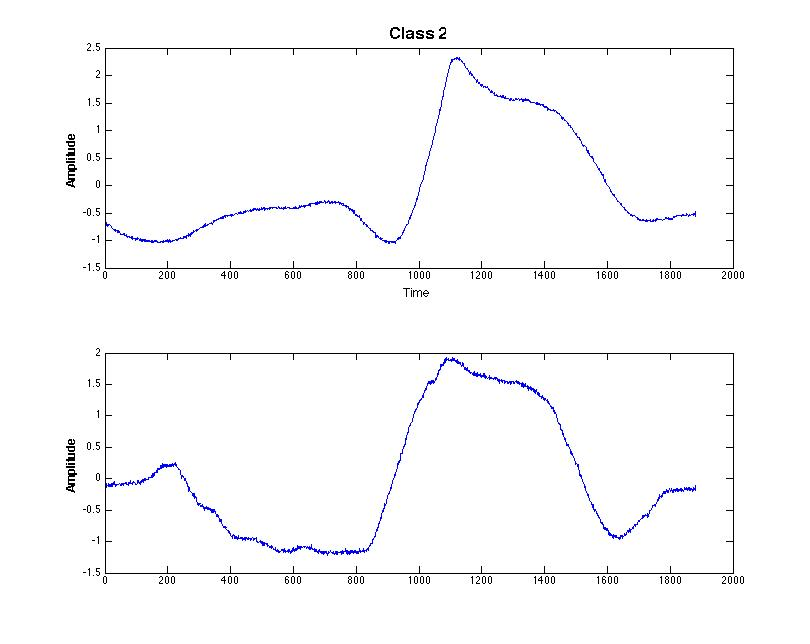
\includegraphics[scale=0.5]{631.jpg}
  \caption{Time series sequences  corresponding to class `2' in the InlineSkate dataset}
  \end{figure}
\section{Wavelet-based Feature Extraction}
\subsection{Background}
The inspiration for the wavelet transform came from the idea of  multiresolution analysis\citep{Chun-Lin2010}. A multiresolution analysis decomposes a signal into a smoothed version of the original signal and a set of detail information at different scales. This type of decomposition is most easily understood by thinking of a picture (can be thought of as a two dimensional signal) and removing from the picture information that distinguishes the sharpest edges, leaving a new image  that is slightly blurred. This blurred version of the original picture is a rendering at a slightly coarser scale. We then recursively repeat the procedure on the smoothed signal. The wavelet transform specifies such a  multiresolution decomposition, with the wavelet functions defining the bandpass filter that determines the detail information and associated with each wavelet is a smoothing function, which defines the complementary lowpass filter.

Mathematically, we can motivate the definition of  the wavelet transform  as follows:

Let  $L^2(R)$ be the set of all  discrete functions with finite energy. Any  discrete function  $f \in L^2(R)$, can be written as a linear combination of translations of the scaling function $\phi(st)$ as shown below:

 $f(t) = \sum_{n=0}^N \alpha_n\phi(st-n)$  where $\phi(st)$ is defined as :
\[ \phi(st)= \begin{cases} 
		1 & \mbox{ if } 0\leq st < 1 \\
		0 & \mbox {otherwise}
		\end{cases}\]	
 Under this representation, the following facts hold.
 \begin{enumerate}[label=\roman{*}]
\item The scaling function is orthogonal to its integer translates i.e
\[  <\phi(st-k),\phi(st-j)>= \begin{cases} 
		1 & \mbox{ if } j==k\\
		0 & \mbox {otherwise}
		\end{cases}\]	

\item As we increase the scale, the support of the function decreases.
\item The subspaces spanned by the scaling function at low scales are nested within those spanned at higher scales. For example if represent $s$ as powers of 2 then: $\phi_{-1}(t)= \phi(2^{-1}t)=\phi_0(t) +\phi_0(t-1)$. 
\end{enumerate}

Before proceeding any further, it is necessary to define the concept of the wavelet. A wavelet \citep{Mallet1998,Zhang2006,Chan1999} is a smooth and quickly oscillating function with good localisation in both  frequency and time. To perform wavelet transformation the Haar function is commonly chosen as the mother wavelet $\psi$. For any scale $s$, the function $\psi(st)$ is orthogonal to  $\phi(st)$.  But like $\phi(st)$, $\psi(st)$  can be expressed in terms of higher order scaling functions $\phi(s't)$ where $s'>s$. Using this knowledge alongside (iii),  the wavelet transformation is applied to  decompose a finite signal $f$  by projecting  $f$  onto  two orthogonal subspaces  $D_1$  and $A_1$of $L^2(R)$ where $L^2(R) = A_1\oplus D_1$. If   $f(t) = \sum_{n=0}^N \alpha_n\phi(st-n)$  then $D_1$ is spanned by  $\{\psi(s't-n)| n\in[1,.. N] \}$ and  $A_1$ is spanned by $\{\phi(s't)| n\in[1,,,N]\}$ where $s'<s$ .

\textbf{Note} :To ensure that $\{\psi(s't-n)| n\in[1,.. N] \}$ forms an  orthogonal basis, the scales are restricted to negative powers of 2\citep{Daubechies1988,Mallet1998}.


 The process is recursive.  After removing the first set of detail information from $f$, we are left with a slightly smoothed version of $f$. We  iteratively remove detail information by applying the transform on the smoothed versions at each scale to progressively extract coarser details of $f$ . We stop the process once we have enough detail information or a smooth enough version to do the analysis we desire. Therefore for given any signal $X$, the wavelet coefficients $H_j(X)$ at any  scale j  can be represented by the series of coefficients  $\{A'_j,D'_j,D'_{j-1}...D'_1\}$.  $A'_j$ represents the coefficients of the scaling function at scale j or in other words it corresponds to the coordinates of  the signal when it projected in the subspace $A_j$. Similarly,  $D'_j...D'_1$ represent the coefficients of Haar wavelet at different scales or in simpler terms, they correspond to the coordinates of the signal when it is projected to  each of the orthogonal subspaces $D_j...,D_1$. 
 To see how this works, lets consider the following example:

Let $f(x)$ be a discrete signal given by $f(x)=\{ 9, 7, 3. 5\}$. This function can be represented as linear combination of the scaling function $\phi(st)$ where s=1. As we have seen in the previous sub section, the wavelet decomposition is a recursive process where at each level j, we project the signal in the two orthogonal subspaces $A_j$ and $D_j$. Since $A_j$ is constructed using the basis $\{\phi (2^{-j}t -n) |n \in [1,..N]\}$  and $D_j$ is constructed using the basis $\{\psi (2^{-j}t- n)|n \in [1,..N]\}$, the wavelet  transform can hence be seen as a series of averaging and differencing operations on a discrete time function. We compute the average and difference between every two adjacent values of the discrete signal $f(x)$.  The recursive procedure to find the wavelet  transform of a discrete function  is shown below.
 
 \begin{tabular}{|c|c|c|}
 \hline \\
 Decomposition Level & Averages & Coefficients\\
  0 &(9 7 3 5) & \\
 1  & (8 4) &(1 -1) \\
 2    &(6)& (2)\\
 \hline\\
 \end{tabular}
 
The level  0  is the full resolution of the discrete function. At the first level of decomposition, (8 4) are obtained by taking the average of (9 7) and (3 5) and  (1 -1) are the differences of (9 7) and (3 5) divided by two respectively. The procedure is repeated on the approximated coefficients (8 4) to obtain (6) and (2) in the next level.





The subspaces $\{A_m\}|_{m=1}^M $ hence satisfy $A_{j+1}\subset A_j$. The details of $f$ at any scale \textbf{m} is a projection of  $f$ onto the subspace $D_M$ and is captured by the coefficients l $D'_M$.  The projection can be represented by the map  $Q_M : L^2(R) \to D_M$ where $Q_M f =\sum_{n=1}^{K} <f,\psi_{Mn}>\psi_{Mn}$( the subspaces $D_M$  are spanned by dilations and translations of the mother wavelet $\psi$). 



Furthermore there exists another operator $P_M$ that maps $f$ to its approximation at scale \textbf{m}:   $P_M: L^2(R) \to V_M\subseteq L^2(R)$. The functional space $L^2(R)$ can therefore be expressed as  $L^2(R)=  \oplus_{m=1}^{M} D_m \oplus A_M$.  where any finite  signal $f \in L^2(R)$ can be expressed as :
\[f(t) = \sum_{n=0}^N \alpha_n\phi(t-n) =P_Mf + \sum_{m=1}^M Q_mf\]

%The wavelet transform is a recursive process. After removing the first set of detail information from $f$ we are left with a slightly smoothed version of $f$. We  iteratively remove detail information by applying the transform on the smoothed versions at each scale to progressively extract coarser details of $f$ . We stop the process once we have enough detail information or a smooth enough version to do the analysis we desire. Once we have decomposed a signal this way, we may analyse the behaviour of the detail information across the different scales(frequency bands). We can extract informations  concerning about the regularity of a singularity which characterises the behaviour of the non-stationary signal at particular point in time. Unlike the fourier transform which is localised only  in frequency, the wavelet transform is localised in both time and frequently(we will see shortly). Furthermore, noise has a specific behaviour across different scales(frequencies). this allows us to  make a clean separation  of the  signal from the noise.
\subsection{Wavelet-based Features }
The wavelet transformation allows a time series sequence to be described in terms of an approximation of the original sequence plus a set of details ranging from fine to coarse. Thus, for given any  time series $X$, the wavelet coefficients $H_j(X)$ at any  scale j  can be represented by the series $\{A'_j,D'_j,D'_{j-1}...D'_1\} \mbox{ where } A'_j$ are the coefficients of the scaling function at scale j and $D'_j...D'_1$ are the  coefficients of Haar wavelet at different scales. The sequence $A'_j$ corresponds to an approximation(smoothed version) of the signal at scale j. The coefficients  $A'_j$ are the \textbf{amplitude} values of the smoothed signal. These coefficients  can be  considered as  global trend descriptors when intra class sequences share the same time aligned global trends. The\textbf{ localised} changes o the other hand are captured in the series of coefficients   $\{D'_j...,D'_1\}$\citep{Zhang2006} where the level of details  captured at each $D_j$ becomes coarser as we move to lower scales.  The decomposition presents \textbf{no loss} of information. Since the wavelet transform is a one to one linear map, the original signal can be fully reconstructed from the approximation part and the detail parts.

The wavelet transformation achieves both time and frequency localisation of a time series. This allows us to analyse singularities specific to both times and frequency bands. The singularities at different frequency ranges are captured by coefficients of  the details and the approximation signals at different scales.  Whereas for signals that are nonzero only during finite spans of time, the wavelet transform has nonzero elements that are concentrated around that time for all scales. This allows us to analyse singularities  localised in different time intervals.  Thus as a feature extraction step, performing wavelet decomposition can be highly advantageous as it allows us to decompose a signal and provide a richer description of its behaviour.  

As we have discussed in the previous section, the intra class sequences in the Cinc\_ECG\_TORSO dataset share similar local and global trends. In such problem domains, the coefficients of both $\psi$ and $\phi$ at different scales are required to form accurate comparison. Figure 7.2  show examples of two instances belonging to class `3' and  two instances belonging to class `4'. From an observation of the plots, it can been seen that apart from sharing global trends, intra class sequences also tend to share similar local trends. Information about the global shape is captured by the coefficients of $\phi$ which behave as global trend descriptors while the  finer details are expressed by the coefficients of $\psi$. Thus, to make accurate comparison, it is necessary to take the coefficients of both $\psi$ and $\phi$ into account.
\begin{figure}[H]
  \centering
      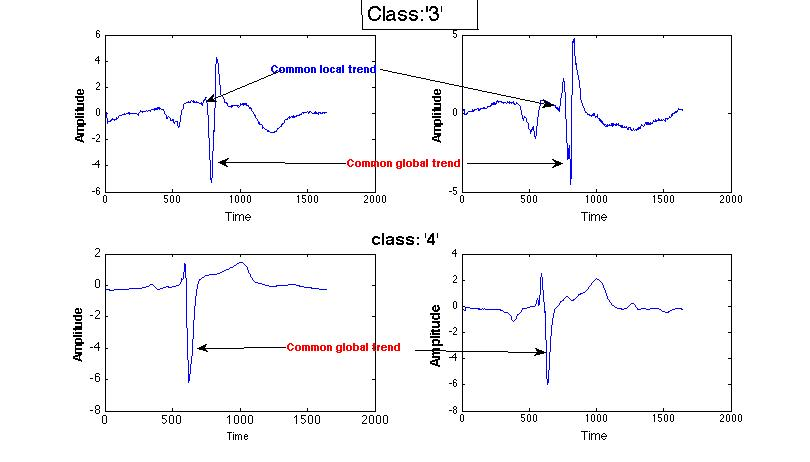
\includegraphics[scale=0.5]{712.jpg}
  \caption{The top two plots corresponds to instances of class `3'  and the bottom two plots correspond to instances of class `4' of the Cinc\_ECG\_TORSO dataset }
  \end{figure}

However, for the the InlineSkate dataset, the global shape is  the only commonality between sequences in the same class. Here intra class sequences  share only  global  similar trends. Figure 7.3 shows examples of samples belonging to the class `2'. The red lines represent smoothed curves fitted to the time sequences to  to capture the overall shape. Both instances share trends that are roughly cubic in nature.
\begin{figure}[H]
  \centering
 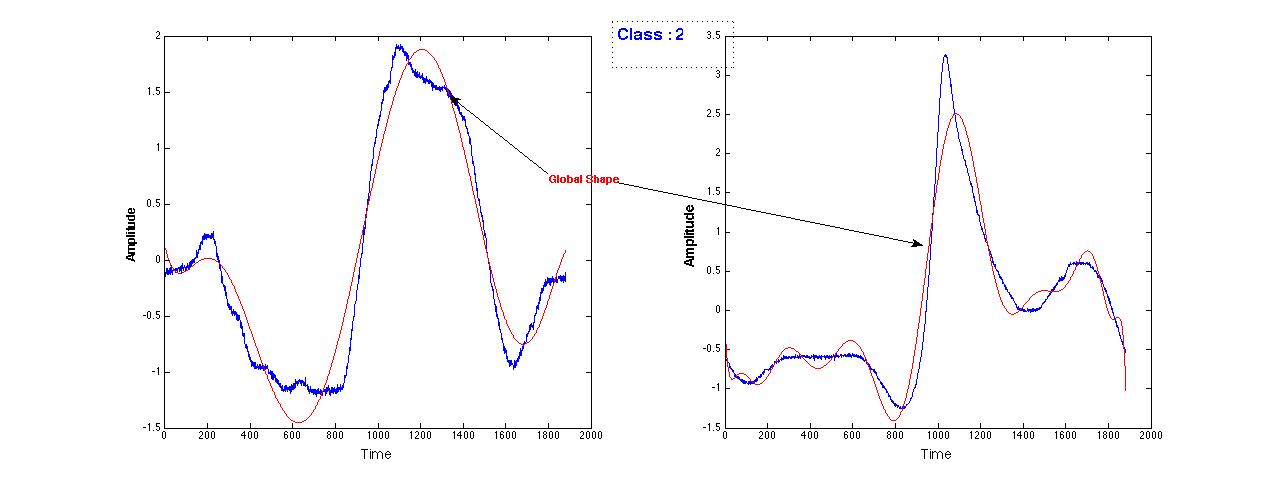
\includegraphics[scale=0.35]{713.jpg}
  \caption{The plots correspond to instances of class '2' of the InlineSkate dataset}
  \end{figure}
In such cases, it can be assumed that the coefficients of $\phi$ play a greater role in discriminating classes than the coefficients of the wavelets.

To investigate whether applying wavelet decomposition prior to SVD as preprocessing step  improves the performance of the 1 nearest neighbour, I conducted the following experiment:
 
 
 \textbf{Datasets}: Cinc\_ECG\_TORSO and InlineSkate
 
 \textbf{Distance metric used}: Euclidean distance
 

 
 \textbf{Preprocessing}: Wavelet decomposition followed by the single value decomposition procedure discussed in 6.3. 
 
 \begin{enumerate}
 \item Step 1: Feature Extraction by applying wavelet decomposition
 
  \textbf{  Cinc\_ECG\_TORSO dataset}: To capture information about both local and global trends with respect to various frequencies and time, I have applied wavelet decomposition up to scale 17. Through experimental testing, I have found that stopping the recursive decomposition at scale 17  is enough to capture the all the  information about the behaviour of  global and local trends at different frequency bands.
  
  Thus, each sequence X is decomposed into the series of coefficients $\{A'_{17},D'_{17}.....D'_1\}$ where  $A'_{17}$ represents the amplitudes of the smoothed signal and $D'_j$ represents the amplitudes of Haar wavelet at scale j. The coefficients of $D'_j$ capture the time localised behaviour of the signal at the frequency band associated with scale \emph{j}. Since the wavelet transform is  a linear one to one mapping, each sequence X is hence mapped to a series of subsequences   $\{A'_{17},D'_{17}.....D'_1\}$ where the sum of the length of the subsequences  is equal to the length of X . The series can be thought of as a sequence of discrete orthogonal signals  where the signal corresponding to index j is constructed by composing the integer translates of the Haar wavelet at scale j i.e $\sum_{n=1}^{K} <f,\psi_{jn}>\psi_{jn}$ with the exception of $A'_{17}$.

 For this analysis, I have omitted the detail coefficients corresponding to scale 1 i.e $D_1$. The reason being  regions in high frequency tend to have a lot of noise embedded in them. Since the first level details capture information about the behaviour of the signal at the highest frequency bands, discarding those details achieves reduction in both the noise  and  the dimensionality of the sequence. Since all sequences in the dataset share the same length and  can be decomposed into the series $\{A'_{17},D'_{17}.....D'_1\}$, discarding $D_1$ reduces the dimension of the time series sequences by half.  
 
 \textbf{ InLineSkate  dataset}: For this dataset,  I have applied wavelet decomposition  up to a depth of  4 levels. Since the commonality of the classes is captured by the global shape. I have only considered the approximation coefficients $\phi$ at scale 4 i.e. the coefficients $A'_4$ . 
 

 \item Step 2: Extracting latent features from wavelet coefficients
 
 As I have mentioned in the previous section, the wavelet  transform can be seen as a series of averaging and differencing operations on a discrete time function.  At the first level, the discrete function is decomposed into  two subsequences \{$A_1$\} and \{$D_1$\} of equal length. The  coefficients of $A_1$ represent the amplitudes of the smoothed signal obtained by averaging every two adjacent values of the original signal. The process is recursive and decomposition is applied again on the approximated signal to separate even more coarser details . Thus after level  j of the wavelet decomposition, we obtain a smooth  signal that is $2^{-j}$ smaller than the original sequence. 
 
 For the InlineSkate and Cinc\_ECG\_TORSO datasets, the sequences within each dataset share the same length. Thus the resultant data matrix constructed using the coefficients extracted from the wavelet decomposition will be full but however in the case of Cinc\_ECG\_TORSO dataset,  the number of columns(this corresponds to the dimension of the data) will be reduced to half, while for the InlineSkate dataset, the number of columns will reduced to $2^{-4}$.  SVD is then applied to each of the data matrix to extract latent features that capture 95\% variation of the data in  the constructed wavelet feature space. 
 
 
 
 \end{enumerate}
 
  The performance of 1NN classifier using SVD and wavelet transform as preprocessing step was compared with  the performance of 1NN classifier using SVD as a preprocessing step and the baseline 1NN classifier. A summary of the results are as follows:


 
 \begin{figure}[H]
  \centering
      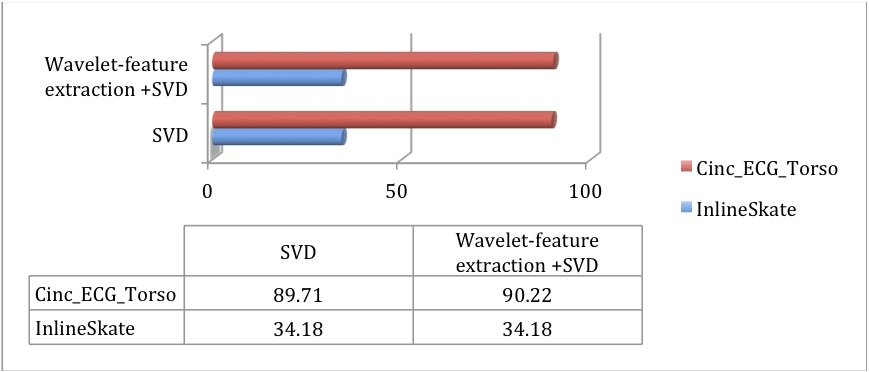
\includegraphics[scale=0.9]{714.jpg}
  \caption{Accuracy}
  \end{figure}
\begin{table}[H]
\begin{tabular}{|c|c|c|c|}
\hline \\
     Dataset  &1NN&1NN+ SVD &1NN+ Wavelet-feature extraction +SVD \\
\hline\\
Cinc\_ECG\_TORSO & 0.88s & 0.77s&0.74s\\
InlineSkate &  1.03s &0.48s &0.45s \\
\hline
\end{tabular}
\caption{Run time in seconds}
\end{table}

\textbf{Observation}
\begin{itemize}
\item As evident from the run time results, applying the  wavelet feature extraction as prior step to SVD reduces the run time of the 1NN classifier even further.

\item For the  Cinc\_ECG\_TORSO data set, removing the detail coefficients of scale 1 i.e $D_1$ leads to a fractional improvement in the accuracy of the 1 nearest neighbour classifier. From this observation, we can deduce two facts:  
\begin{enumerate}
\item Because  the accuracy has not decreased, we can conclude that the information contained in the finer details of sequences present redundant information.

\item Removing such information has the affect of  decreasing  the intra class variance as evident from the increase in accuracy.

\end{enumerate}

\item  In the case of the InlineSkate data set, considering only the approximation part of signal i.e $A_4$ results in no decrement in the accuracy of the 1 NN classifier. This shows that when comparing sequences using the euclidean metric, the details in the first 3 levels: $D_3,D_2 $ and $D_1$ play no role in the classification process. To investigate whether applying further wavelet decomposition can improve  the accuracy of the classifier, I repeated the experiment for the InlineSkate dataset again but this time  I have considered  the coefficients of $A_5$(the approximation of $A_4$)and $A_6$(the approximation of $A_5$). A summary of the results is given below:

 \begin{table} [H]
 \centering
\begin{tabular}{|c|c|c|c|}
\hline \\
   Dataset   &Using $A_6$ & Using $A_ 5$& Using $A_4$\\
\hline\\
InlineSkate &  33.82 \%&34.18\%  & 34.18\%\\
\hline
\end{tabular}
\caption{Accuracy results}
\end{table}
\begin{itemize}
\item Discarding  coarser details from the approximated signal  $A_4$ decreases the accuracy of the 1NN classifier as we increase the number of decompositions. This shows that for this dataset, we cant achieve any improvement in the accuracy of the 1NN classifier by considering approximations from further decompositions using the wavelet transform.

\end{itemize}

\end{itemize}

The subsequence $A_j$ as I have mentioned before corresponds to an approximation(smoothed version) of the signal at scale j. The coefficients of $A_j$ are the amplitude values of the smoothed signal. These coefficients   are constructed by averaging every two adjacent values of the approximated signal corresponding to j-1 and  can be  considered as  global trend descriptors when intra class sequences share the \textbf{same} time aligned global trends. 

From the analysis above, replacing the original sequences with the smaller approximated sequences $A_j$  doesn't improve  the accuracy of the 1NN classifier for   the InlineSkate dataset. And in fact, the accuracy of the classifier decreases when we consider approximations from the lower scales i.e  j $>$4. Thus, we can conclude  that the global trends shared by intra class sequences are not localised with in the \textbf{same} intervals of time.  Metrics such as the euclidean will  be hence inept in utilising the embedded information about the global shape as they are  constrained to conducting  only linear matches between  temporal dimensions of sequences

However, for datasets in which intra class sequences  share the same time localised/aligned global trends, we can expect that by applying the wavelet decomposition as a preprocessing step and considering the approximated part of the signal at a scale j, the accuracy of the baseline 1NN classifier can be improved. To  verify this assertion, I performed an additional experiment  on the UCR dataset 'Synthetic Control'. This dataset have been chosen because experiments have shown\citep{Xie2010} that the intra class sequences of the dataset are linked with each other through time aligned global trends.



 
 
\textbf{Preprocessing Steps}

The dimension i.e the length of the time series sequences is 60 which is very small. Hence the wavelet decomposition has been applied only up to level 1 i.e only the coefficients of $A_1$ are considered. The application of SVD was deemed not necessary for this dataset since the sequences have very small lengths.

The performance of 1NN classifier using  wavelet transform as a preprocessing step was compared with  the performance of the baseline 1NN classifier and the performance of the  1NN classifier combined with the DTW metric. A summary of the results are as follows:


 \begin{table} [H]
 \centering
\begin{tabular}{|c|c|c|c|}
\hline \\
   Dataset   & 1NN +Euclidean & 1 NN +Euclidean + Wavelet&1 NN +DTW\\
\hline\\
Synthetic control &  0.32s & 0.30s  & 777.3s\\
\hline
\end{tabular}
\caption{The run time}
\end{table}


\begin{figure}[H]
  \centering
      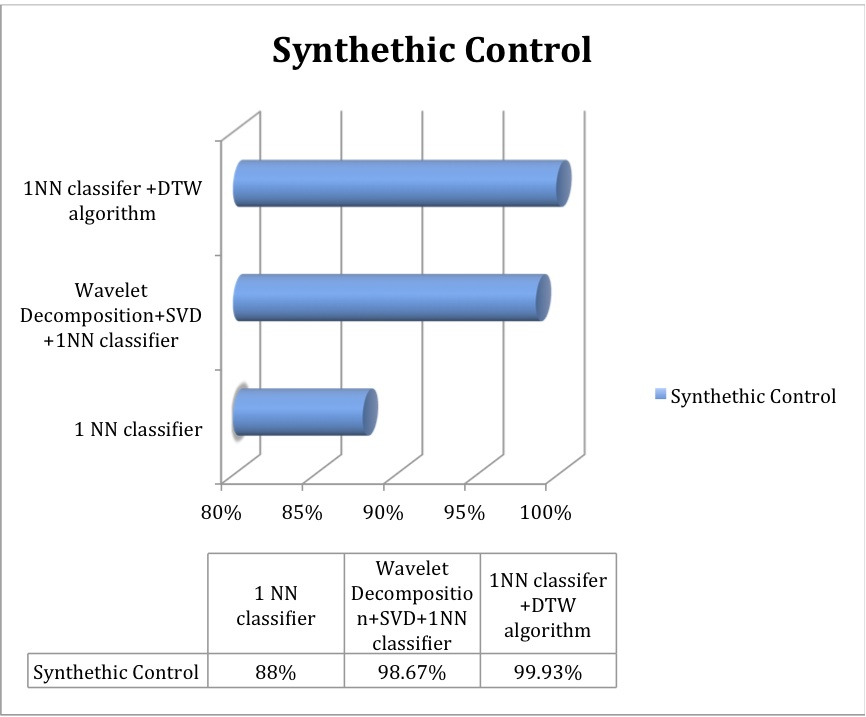
\includegraphics[scale=0.7]{724.jpg}
  \caption{Accuracy}
  \end{figure}
  
 
\textbf{Observation}
\begin{itemize}
\item Removing unnecessary details by smoothing the signals improves the accuracy of the 1NN classifier by 10\%. The resultant accuracy is  identical to the best accuracy achieved by combining 1NN classifier with the DTW algorithm. Furthermore, the run time of 1NN classifier using the Euclidean metric is $10^4$ times smaller than the run time of the 1NN classifier combined with the DTW metric.

This proves  that by applying the  wavelet transform as a preprocessing step, the 1NN equipped with the Euclidean metric can identify intra class sequences that  roughly share the same time aligned global trends with  high accuracy without being subjected to high run times.

 
\end{itemize}



\section{Curvature-based Feature extraction}
In the previous section, we have observed that for datasets such as  the InlineSkate dataset, the main commonality between intra class sequences is the global shape. Applying wavelet decomposition and considering only the approximation part of the signal $A_4$  allows us to achieve dimensionality reduction but without any improvement  in accuracy. The low accuracy achieved by the classifier  is primarily due to the limitations incurred in comparing sequences  using the euclidean metric. The individual amplitude values on their own are not reflective of the global shape of the sequence. This creates  the motivation to explore feature extraction methodologies that capture information about the shape of the sequence.

To address this issue, I propose the following  multi step feature extraction methodology to extract useful features from the InlineSkate dataset:
\begin{enumerate}[label=\roman{*}]
\item  Apply wavelet decomposition up to scale j and consider only the approximation part of the signal $A_j$. This achieves dimensionality reduction by  pruning away unwanted details while preserving information about global trends.
\item  Replace the amplitude value associated with each point of the approximated signal with curvature value of the smoothed signal associated with the corresponding point(details to follow).
\item  In the scenario  where the  sequences extracted  using the wavelet transform still posses very high dimensionality,  apply the  fourier transform and consider only the first half of the fourier coefficients(details to follow).

\textbf{Note}: This step should  only considered when we are working with time series datasets that have very high dimensionality.
 
\item If the dimension of the extracted fourier feature space  $\gg$ than the number of samples after the first 3 steps then apply SVD on the result sequence of fourier feature descriptors to extract a smaller set of latent vectors that capture the 95\% variation of the feature vectors in the fourier feature space. 

In the following sections, I  provide  a detail description of the procedures specified in step (ii) and step (iii) of my proposed methodology. 


\end{enumerate}

\subsection{Motivation for curvature based features}
Replacing the individual  amplitude values with the curvature estimates of the corresponding points  can allow  the euclidean metric to take into account the \textbf {shape} of the signals at the corresponding points  when conducting a linear match. The curvature of a geometric object is a  quantitive description of the shape of that object\citep{Adnan}.  It dictates the amount by which a geometric object deviates from being flat or straight. 
Formally, the curvature of a curve can be defined  as follows:

Let $\gamma$ be a differentiable curve on  $\textbf E^3(\mbox{Euclidean Space})$ such that 
	\[ \gamma : (-\epsilon,\epsilon) \to U \subseteq \textbf E^{ 3} \] 
	\[ \gamma(t) =\left ( \begin{array}{c}
	                                    x(t) \\
	                                    y(t) \\
	                                    z(t) \end{array}  \right) \]
 The derivative of this function  $ \gamma'(t) =\left ( \begin{array}{c}
	                                    x'(t) \\
	                                    y'(t) \\
	                                    z'(t) \end{array}  \right) $ is the velocity of this curve.  	                                  
	                                    
	                                    Thus by assuming that this curve is parameterised by arc length (i.e. the curve is parameterised to have unit velocity $\| \gamma'(t)\| =1 $ ) we define the \emph {curvature}  of as curve
	                                    as  \[\kappa = \| \gamma''(t)\| \]
	             which in fact is none other than the magnitude of the acceleration of a curve.

Geometrically  one can imagine  $\kappa$ as a  parameter determines the amount of the bending of that the curve experiences in the flat euclidean space.



\subsection{Extracting curvature based features}
To extract features that capture the \textbf{ shape} of the dominant trends in a sequence, I performed  the following two step feature extraction process.

\textbf{Step 1: Extraction of curvature estimates}

  To compute the  curvature estimates at each point in a  time series sequence, I  have fitted a \textbf{smoothed cubic spline} to each sequence. A spline is a   polynomial function that is piecewise-defined, and possesses a high degree of smoothness at the places where the polynomial pieces connect \cite{Boor1978}. A cubic spline is a  specific type of spline which is  constructed using piecewise  polynomials of order 3. 
 
Although applying the wavelet decomposition reduces the degree of noise, fitting a cubic spline directly on the sequences  will still not be ideal as the approximated signals may still have jagged regions as shown by figure 7.6. The figure shows the approximated  signal and its associated fitted curve of an instance in the InlineSkate dataset. To overcome this issue, I have thus applied smoothed cubic spline to fit smooth curve to each sequence(given by the blue plot in figure 7.6) .
  
\begin{figure}[H]
  \centering
      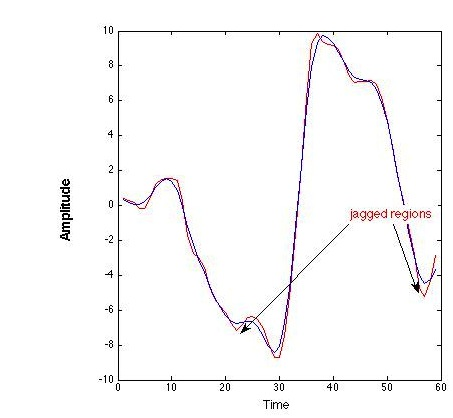
\includegraphics[scale=0.6]{725.jpg}
  \caption{The red plot corresponds to the approximated signal $A_4$ and the blue plot corresponds to the fitted cubic spline }
  \end{figure}

  
 Mathematically, the smoothing spline estimate $\hat g(x)$ of the actual function $g(x)$ is defined to be the minimiser of :
\[
\lambda \sum_{i=1}^n \{ y_i - \hat g(x_i) \}^2 + (1-\lambda) \int_a^b \{\hat g''(t)\}^2 \,
dt
\]
where  $\lambda \in[0,1]$

\begin{itemize}
\item As $\lambda \to 1$,the smoothing spline converges to the interpolating spline. 
\item As $\lambda \to 0$,the roughness penalty becomes paramount and the estimate converges to a linear least squares estimate.
\end{itemize}

The critical parameter here is $\lambda$ and it's value determines the nature of the fit. For the sequences in the  InLineSkate dataset, exact fitting is unnecessary as the sequences have jagged regions in them. Ideally, we want to choose a value of  $\lambda$ that allows the estimated curvatures to directly correlate with significant events/trends in the time series sequence. 

 For my analysis, I have chosen the value of 0.2.  Through conducting experiments, I have observed that  setting $\lambda$ to this value allows the computed curvatures to reflect significant events in the time series sequence. An illustration of this can be seen  in figure 7.7. The plots correspond to an instance of class '7' from the InlineSkate dataset. The left hand plot corresponds to the approximated signal $A_4$ extracted through wavelet decomposition  while the righthand plot represents   the curvatures computed at each of the time stamps. From the observation of the figure, it can be seen that the computed curvatures do reflect information about significant events in the time series sequence. For instance the peak value on the curvature plot at t=148  is in accordance with the sharp bend of the signal at that time.
 
 \begin{figure}[H]
  \centering
      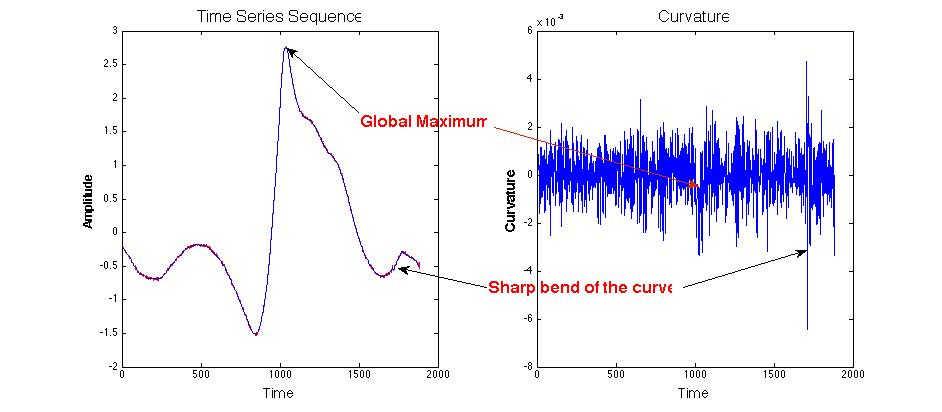
\includegraphics[scale=0.5]{721.jpg}
  \caption{The left hand plot represents the time series sequence while the right plot corresponds to curvatures computed at each point in the time series sequence}
  \end{figure}
  The curvatures $\kappa$ at each point of the fitted smooth cublic curve is computed using the following expression:
  \[ \kappa =\frac{\hat g^{"}(x)}{(1+\hat g^{'}(x)^2)^\frac{3}{2}}\]
  
  \textbf{Step 2: Extract features that reflect the global shape}
  
  The main objective here is to extract features that reflect the \textbf{global} shape of the time series sequence.  Although applying the wavelet decomposition reduces the dimension (i.e the length) to $\frac{1}{16}$ of the original length, the resultant sequences especially in the case of \textbf{high} dimensional time series sequences may still be long enough to retain some local trends. The above mechanism embeds  the  information of local curvatures to each point of the time series sequence. Hence for datasets where intra class sequences are connected by just by global trends, the curvature associated local trends may increase the intra class variance. 
  
  What we are really interested in is in the extraction of  global shape descriptors. The shapes of the global trends  of  a signal are preserved in the low frequency bands while the  higher frequency bands encode information of local  shapes \citep{Osowski2002}. Thus, to extract global shape descriptors, I have applied the discrete fourier transform\citep{Bracewell1986} on the extracted curvature  sequences. 
  
The Fourier transform maps time into frequency and phase. For each frequency the fourier transform yields an amplitude and a phase value. Thus, the transform captures the behaviour of the signal at different frequency band. Since the amplitudes represent curvature values estimated at step 1, the fourier transform therefore capture the behaviour of the \textbf{shape} of the signal  at different \textbf{frequency} bands.  The curvature-sequences can now be represented as the sum of sine and cosine  waves whose phase and `amplitude' are given by the fourier transform.
 
 For any time series sequence, the coefficients of the discrete fourier transform for each frequency band is computed as follows:
  \[  X_k =\sum_{i=1}^n x_n.e ^{-2\pi i k\frac{n}{N}} \]
  
 To extract global shape descriptors only the magnitudes of the fourier coefficients have been used, Since  global trends \citep{Mallet1998,Osowski2002} are preserved in the lower bands,  only the first few fourier coefficients have been considered. For the InlineSkate dataset, I have only selected the first 116 coefficients as features for nearest neighbour classification.  Since the number of fourier coefficients is smaller than the number of samples, for this dataset, the 4th step i.e SVD was deemed not necessary.
 

 
 To investigate whether using  the 3 step feature extraction method  improves the accuracy of the 1 nearest neighbour classifier, I re-ran the experiment again on the InlineSkate  dataset but using the proposed feature extraction method as a prior preprocessing step. The details of the conducted experiment are as follows:
 
 \subsection{Experiments}
 
 \textbf{Dataset used:} InLineSkate dataset
 
 \textbf{Preprocessing step}
 
\begin{figure}[H]
  \centering
      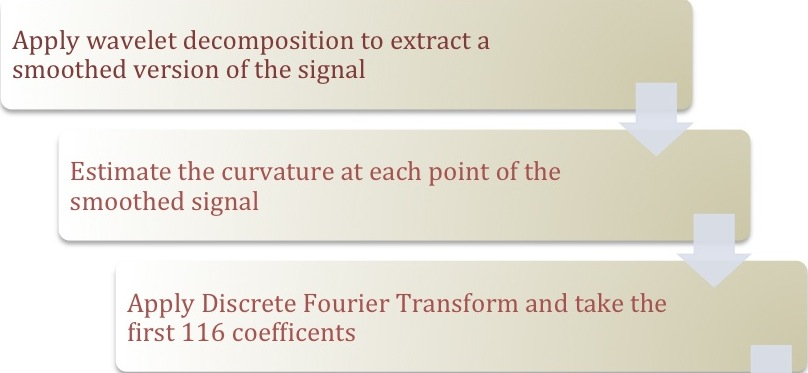
\includegraphics[scale=0.8]{722.jpg}
 
  \end{figure}
   \textbf{Note}: Dimensionality reduction occurs at step 1,3 and 4. Redundant features are pruned away at this steps to finally result a small set of latent factors that be used to cluster/classify inter class sequences that are distinguished by global trends. However, to choose the appropriate number of fourier coefficients, the experiment was repeated multiple to decide the optimum number of fourier coefficients that yields the highest accuracy. Thus as a result, the run time incurred during preprocessing was around 187s. I will discuss this issue further in the discussion section.
 
After selecting the appropriate number of fourier coefficients to use, the experiment was  run  once again.  The run time and accuracy of the  1NN classifier  was compared with  the performance of the baseline 1NN classifier and the performance of the  1NN classifier combined with the DTW metric. A summary of the results are as follows:



  
   \begin{figure}[H]
  \centering
      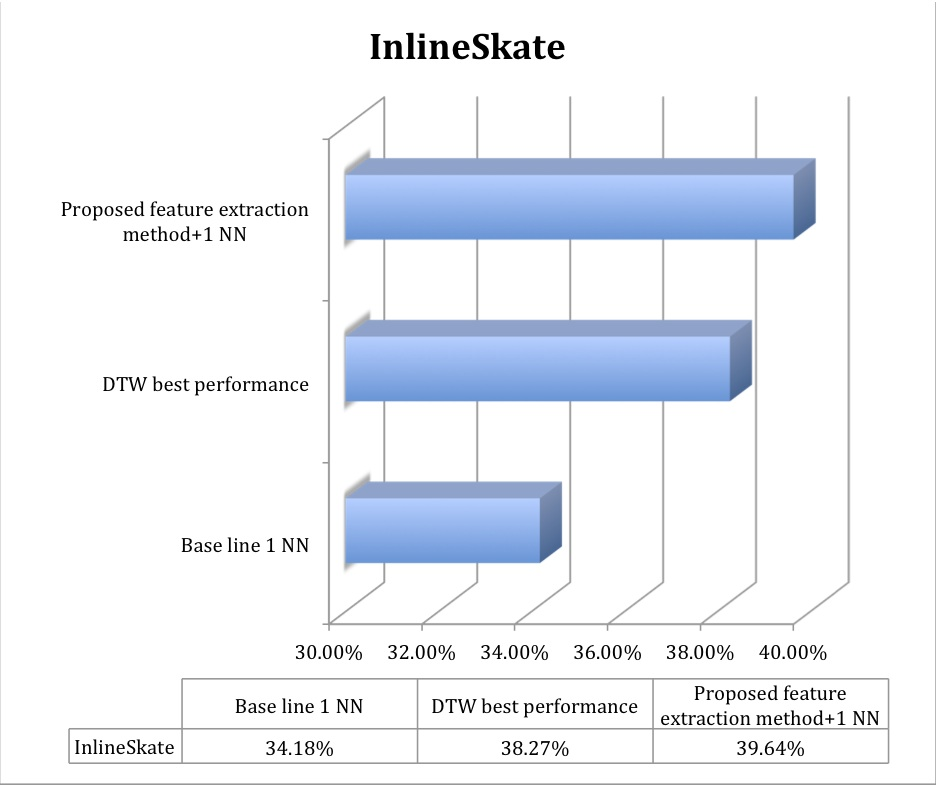
\includegraphics[scale=0.7]{723.jpg}
 \caption{Accuracy}
  \end{figure}
 
 \begin{table}[H]
\scalebox{0.6}{
\begin{tabular}{|c|c|c|c|}
\hline \\
 Dataset  & 1NN +Euclidean distance &1NN + Euclidean distance +proposed feature extraction method & 1NN +DTW metric\\
\hline\\
InlineSkate & 1.03s & 0.199s & 3.290 $\times 10^6$ \\
\hline
\end{tabular}}
\caption{Run time}
\end{table}

 \textbf{Observations}
 \begin{itemize}
  \item Embedding the baseline 1NN classifier with the proposed feature extraction method reduces the run time of the  the baseline classifier by an order of 9. This is expected as we achieve dimensionality reduction in step 1 and step 3 in the feature extraction phase.
  
   \item The extracted   shape descriptors are more successful in capturing information about the global shape than the raw amplitude values. Embedding the baseline 1NN classifier with the proposed feature extraction method allows the Euclidean metric to be as effective as the DTW metric when the DTW is   employed on the raw sequences. From the table above, it can be seen that the 1NN classifier's accuracy has improved by  5.46\% and  is now identical to the accuracy of the classifier using   DTW algorithm on the raw sequences.. Furthermore, the run time of 1NN classifier using the Euclidean metric is $10^7$ times smaller than the run time of  the 1NN classifier combined with the DTW metric.
    \end{itemize}
    
    
As we have discussed in the previous section, for time series sequences, the DTW algorithm makes a richer comparison than the euclidean metric. By warping the time axis, the DTW algorithm compares each point in one sequence with points at different temporal regions in the second sequence. The euclidean metric on the other hand is only restricted to conducting linear matches between the temporal dimensions.  However from the  experimental results, it can be seen that for  the InlineSkate dataset, if we embed the proposed 3 step preprocessing method then  the performance of  using euclidean metric is equivalent to applying the DTW algorithm  on the raw sequences.

To  verify that the proposed feature extraction method is not tailored for this particular time series dataset, I conducted a separate  experiment on the UCR dataset CBF\citep{UCR} dataset. The �CBF� dataset have been chosen because experiments have shown\citep{Xie2010} that the intra class sequences of the dataset tend  share the same global trends.  

\textbf{Setup}:
\begin{itemize}
\item From examining the plots of the time series sequences, I have observed that appyling wavelet decomposition only up to level 3 is enough to remove the local trends. Thus, I have   taken the coefficients of the approximated signal $A_3$.
\item  For the curve fitting phase, by visually comparing the corresponding fits,  I have observed that setting $\lambda$ to 0.35 gives the best  smoothed fit without interpolating the jagged regions of the sequences .
 
\item  Since the length of the sequences is only 128, the information of individual local trends  is almost pruned away in the early levels of the decomposition. Figure 7.9 shows the plot of a raw signal corresponding to an instance of class`3' from the CBF dataset  and the  signal constructed from approximation $A_1$ using the reverse wavelet transform \citep{Mallet1998}. From the figure, we can see that  almost the jagged portions of the signal are smoothed away when we stop the decomposition at the first level.
Thus, when we repeat the wavelet decomposition 3 times and take $A_3$, we can expect the coefficients of $A_3$ to correspond to a smoothed signal where  all the local trends are pruned away. The length of the $A_3$ is now 8 times smaller than the original sequence, therefore, the fourier extraction step was deemed not necessary in this case as the extracted sequences are very small in length. 

\end{itemize}
  
  
  \begin{figure}[H]
  \centering
      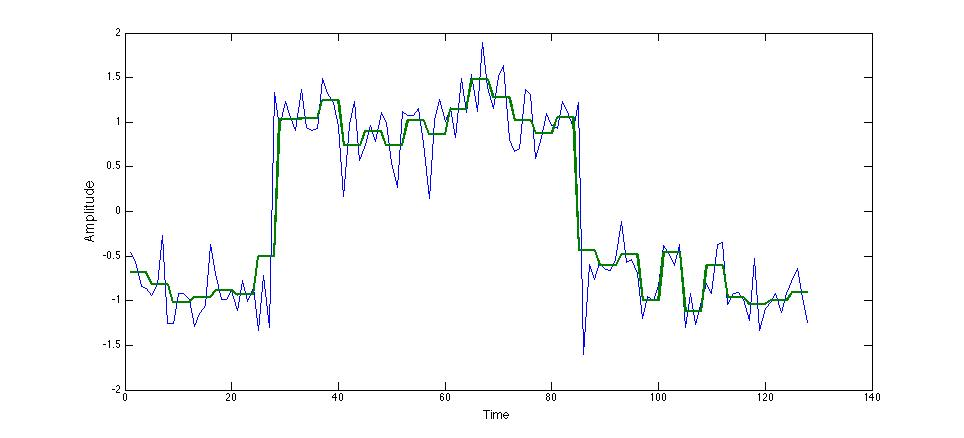
\includegraphics[scale=0.5]{726.jpg}
 \caption{The green plot corresponds to signal constructed from $A_1$ and the blue plot presents the original signal }
  \end{figure}
 The accuracy of the model was compared against the accuracy of the baseline 1NN classifier and the  best accuracy of 1NN classifier using the DTW algorithm\citep{Xie2010}.
 
A summary of the results are as follows:


 \begin{table} [H]
 \centering
\begin{tabular}{|c|c|c|c|}

\hline \\
  Dataset   & baseline 1NN  & 1NN + proposed  method & 1NN + DTW algorithm\\
\hline\\
CBF &  85.2\%&95.78\%  & 99.92\%\\
\hline
\end{tabular}
\caption{Accuracy results}
\end{table}

\begin{table} [H]
 \centering
\begin{tabular}{|c|c|c|c|}

\hline \\
  Dataset   & baseline 1NN  & 1NN + proposed  method & 1NN + DTW algorithm\\
\hline\\
CBF &  0.109s & 0.094s  & 1048.2s\\
\hline
\end{tabular}
\caption{Run time results}
\end{table}
Observation
\begin{itemize}
\item Augmenting the baseline 1NN classifier with the proposed multi-step feature extraction process improves both the run time and accuracy of the algorithm. The classifier achieves an improvement of over 10\% in accuracy and incurs a run time which is 9 times smaller than its baseline implementation. Replacing the Euclidean metric with the DTW metric allows the 1NN classifier to achieve almost perfect accuracy on the raw sequences  but at the cost of high run time. Thus by using  the proposed feature extraction step, we can achieve improvement in both run time and accuracy. 

\end{itemize}



\section{Conclusion}

 To summarise, in this chapter we investigated methods to  improve the accuracy of 1NN classifier when it employs  the Euclidean metric on time series datasets. In section 7.1, we have observed that applying the wavelet transform as a preprocessing step to extract coefficients can improve the identification of  intra class sequences that roughly share the same time-aligned local or/and global trends. Whereas in the later chapters, we have observed that for time series datasets where intra sequences share a global shape,  applying the preprocessing strategy proposed in section 7.2 can help the euclidean metric to be as equally effective as a DTW metric when classifying sequences without being subjected to high run times.
 
 
  
  
  
  \chapter{Adapting The Euclidean Metric To Perform  Isolated Word Recognition}
  
  In chapter 1, we have seen that one of the main limitations of applying the Euclidean metric in time series domains  is its inability  to handle sequences that vary in length. For time series sequences such as speech utterances, sequences belonging to the same class may vary in terms of speed, time duration and scale as a result of different speakers, the spoken context  etc. Hence, classifying sequences based only on a linear match of their  temporal dimensions wont work in such scenarios.  To address this issue, in this  chapter, I primarily focus in  exploring feature extraction methods that identifies and extract useful features that can be used to distinguish sequences of different classes. Mapping each sequence to the well chosen  constructed  K  dimensional feature space can increase the inter class variances of sequences and at the same time ensure that  all sequences share the same length. This provides  the context for the Euclidean metric to be applied on classifying the data sequences.  
  
 \section{Identifying the acoustic signature of individual digits}
 Speech utterances associated with the same lexical identity  will  fundamentally  share strong  acoustic  properties that allows a listener to recognise them to be part of the same class. With the exception of homophonic word pairs, individual words can be purely differentiated in the way they sound.  For example, the word `and'  and the word `the' have totally different sounds even if they are spoken in different contexts or by different speakers. Therefore, for datasets such as the TIDIGITS corpus where the vocabulary doesn't consist of any homophonic word pairs, we can hypothesize that each lexical identity will have a unique acoustic signature.
 
 To verify this hypothesis, I conducted exploratory data analysis to identify visual commonalities between  intra class sequences.  Figure 8.1 shows examples of utterances corresponding to digit 7 of the TIDIGITS corpus. Both plots differ in their behaviour with respect to time localised events. The left hand plot has a region with low amplitudes between t=4000 and  t=5000 but this property  is absent in the right hand plot.  However, even though the signals tend to posses different acoustic properties they share very  similar envelopes.   From visually comparing the plots of instances of other classes, I have observed that the shape of the envelope is indeed the key attribute that helps us to identify plots of the same lexical identity. Thus, for the remaining part of this chapter, I will concentrate on constructing feature extraction that capture information about the shape of the envelope of the signals.  
  
 
  \begin{figure}[H]
  \centering
      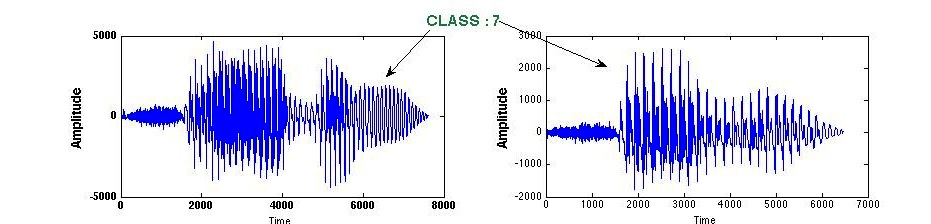
\includegraphics[scale=0.5]{81.jpg}
 \caption{Instances of class 7 }
  \end{figure}

\section{Homogenising the dimensionality of speech utterances}
 Since speech utterances do not share the same length, their respective envelopes will also differ in sizes. This makes it impossible for metrics such as the Euclidean distance to compare  envelopes of different utterances just by a linear match of their temporal dimensions. Hence, this provides the motivation to explore mappings that preserves the shape of the envelopes while restricting them to share the same size.
 
 An obvious strategy will be to scale all the speech utterances to share the same length. To rescale the speech utterances, I have applied the \emph{matlab} function \emph{resample}   that resamples each sequence  $\frac{P}{Q}$ times the length of the  original sample rate using a polyphase implementation\citep{Shahana2007}. Figure 8.2 shows the plots of an instance of class `1' and its resampled version. From the observation of the figure, we can clearly see that the envelope of the speech utterance is preserved after the signal has been rescaled to a fixed length. For my analysis I have chosen P to be mean length of the utterances in the training set and Q to be an adaptive parameter which is set to the length of each individual sequence. This ensures that all utterances are rescaled to share the same length which in this case is the mean length of the utterances. Having  now resolved the dimensionality issue  that previously prevented the Euclidean metric from acting on speech datasets, the next step is to investigate feature extraction methods that can capture information about the shape of the envelopes.
  
   \begin{figure}[H]
  
      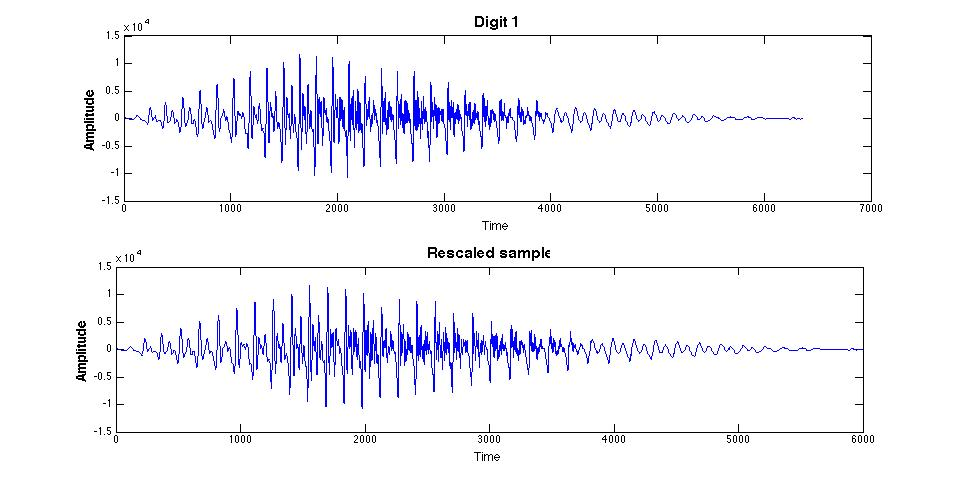
\includegraphics[scale=0.5]{82.jpg}
 \caption{The top plot represents  to a  raw utterance belonging to  digit 1 while  the bottom plot corresponds to a rescaled version of the raw signal  }
  \end{figure}

\section{ Feature extraction methods to construct acoustic fingerprints}

The objective now is to construct a feature extraction scheme that captures information about the shape of the envelope  associated with each speech utterance. This problem is very similar to the problem we addressed in the previous chapter. To remind the reader, in the previous chapter we explored curvature-based feature extraction methods that capture information about the global shape of time series sequences.   In comparison, the current problem only differs in the fact that instead of looking at the entire signal, we are only interested  in the shape of the envelope of the signal. Thus, if we find a procedure to extract the envelope associated with a  signal, then we can use the multi step feature extraction methodology proposed in section 7.2 to extract the curvature based features that capture the shape of the envelopes.

\subsection{Extracting the envelope of a speech utterance}
To separate the envelopes from their respective  speech utterances, I have applied the Hilbert transform\citep{Feldman1997}. 

\textbf{Brief description of the Hilbert Transform:}

The Hilbert transform of a function f(x) is defined by:

\[f(t)=\frac{1}{\pi}  \int_{-\infty}^ {\infty} \frac{f(x)}{(t-x)} dx\]
Theoretically, the integral is evaluated as a Cauchy principal value\citep{RamP.Kanwal1996}. The above integral can be thought of as   the  convolution of the function $\frac{1}{\pi t}$ with the function f(t) :
\[F(t) = \frac{1}{(\pi t)}  f(t)\]

Intuitively speaking, the   transform can  be considered to be a filter which simply shifts phases of all frequency components of its input by $\frac{-\pi}{2}$ radians. Using the  Hilbert transform, we can construct  an "analytic (complex time) signal Y(t)  such that:
\[Y(t) = y(t) + j h(t)\]
 where y(t) corresponds to the original signal and h(t) corresponds to the Hilbert transform of the original signal.

To extract the envelope e(t) of a signal x(t) , we  consider only  the magnitude of this analytic signal as shown by the following equation.

$$e(t) = \sqrt{x({t})^{2} + \hat{x}(t)^{2}}$$


where $\hat{x}(t)$ is the Hilbert transform of x(t).

Figure 8.3 provides an illustration of the envelope extraction process. The topmost plot corresponds to an instance of digit `2' from the TIDIGITS corpus. The second plot corresponds to the envelope of the raw signal.  If we represent each raw signal as an image than the envelope of the signal will correspond to its perimeter of the image which is simply  the outline of the upper and lower parts of the signal. Hence, to capture the envelope, the outlines of both the upper part and lower part  of the signal must be captured. To achieve this, I  applied the Hilbert transform twice: once on the positive part of the signal to extract the top envelope and next on the negative part of the signal to extract the bottom envelope. The second plot in figure 8.3  represents the augmentation of the  upper and lower envelopes of the speech utterance. However this extraction procedure is not `clean'.  As evident from the figure, the extracted envelopes  have very high frequencies which is expected  since human speech is spoken at a very high frequency.   To remove these unnecessary details, I performed wavelet decomposition to extract a curve that captures the envelope of the utterance. The bottom plot corresponds to the envelope reconstructed  using just the coefficients of the approximated part of the wavelet transform. 

\begin{figure}[H]
  
      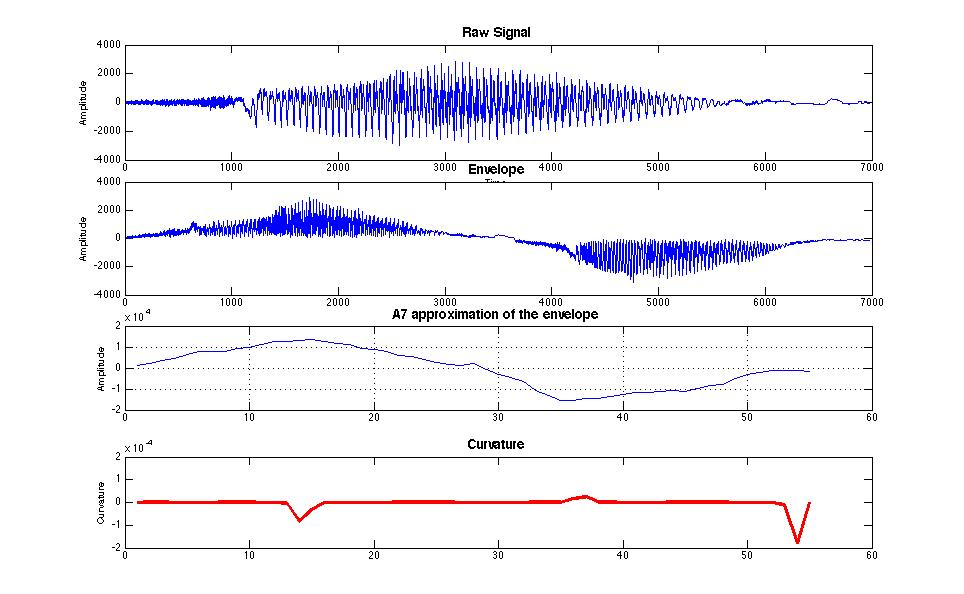
\includegraphics[scale=0.4]{83.jpg}
 \caption{The top plot corresponds to an utterance of digit 5. The second plot corresponds to the envelope of the signal extracted by the Hilbert transform. The third plot corresponds to a smoothed version of the envelope extracted by wavelet decomposition   }
  \end{figure}
  
  \section{Experimental Results}
  
  By combining the envelope extraction method with the feature extraction methods discussed in section 8.2, we now have a methodology to extract  features that captures the shape of the envelopes of a signal. To test this idea, I have conducted the following experiment:
  
  \textbf{Dataset}: The TIDIGITS dataset
  
  \textbf{Distance metric used}: Euclidean distance.
  
  \textbf{Preprocessing steps used}:
 
 For each utterance:  
  \begin{itemize}
 \item Apply the matlab function `resample' to rescale the utterance to the mean length of the sequences in the training dataset. This ensures that  all sequences to share the same length while at the same time preserving the shape of the envelopes associated with each utterance.  
  \item  Apply the Hilbert transform to extract the envelope associated with the speech signal.
  \item Apply the wavelet transform can remove the  unnecessary details  from the extracted envelopes.  The envelopes extracted through the Hilbert transform contain regions with very high frequencies.  This is expected  as human speech is spoken at a very high frequency . Using the wavelet transform, we can recover the global trend of the envelope by  smoothing away the regions with high frequencies.  For this problem, I stopped the wavelet decomposition at level 8 and considered only the approximated coefficients $A'_8$.  Through exploratory data analysis, I have found this level is in fact the minimum level of decomposition that needs to be applied to extract a curve that captures the envelope of the signal. The extracted envelope is hence replaced by the smoothed envelope corresponding to the  approximation coefficients $A'_8$.
  \item Fit a smoothed spline to each extracted envelope  and replace the amplitude values associated with each point of the fitted spline with  the local curvatures associated with those points.  
    
  \item  The fourier  feature extraction phase along with SVD was deemed not necessary since the wavelet decomposition reduces the length of the signals by $2^7$. 
  
  
  %The extracted sequences however, still suffer from very high dimensionality.  Since the  objective here is to extract the global shape of the envelope, by  following the methodology discussed in 7.2.2, I have taken the first k fourier coefficients from the fourier transform  of the signal.  As I have already mentioned in the section 7.2, the  information of the global shape is captured by the fourier coefficients of the lower frequencies\citep{Osowski2002}. For this dataset, by conducting multple experiments, I have found that taking the first 77 fourier coefficients yield the highest results.
   \end{itemize}
\textbf{Run time of preprocessing}  : The time taken to apply this above feature extraction methods is 106.5s. 


To investigate whether the proposed feature extraction methodology improves the performance of the 1NN classifier, I have compared  the accuracy and the run time of the classifier against the performance achieved by  the  baseline 1NN classifier combined with SVD when its employed on the rescaled speech utterances. A summary of the results are as follows:
 \begin{table} [H]
 \centering
\begin{tabular}{|c|c|c|c|}

\hline \\
 baseline 1NN + SVD & 1NN + multi step feature extraction method \\\\
\hline\\
   56.5s & 5.23s\\
\hline
\end{tabular}
\caption{Run time results}
\end{table}

\begin{figure}[H]
  \centering
      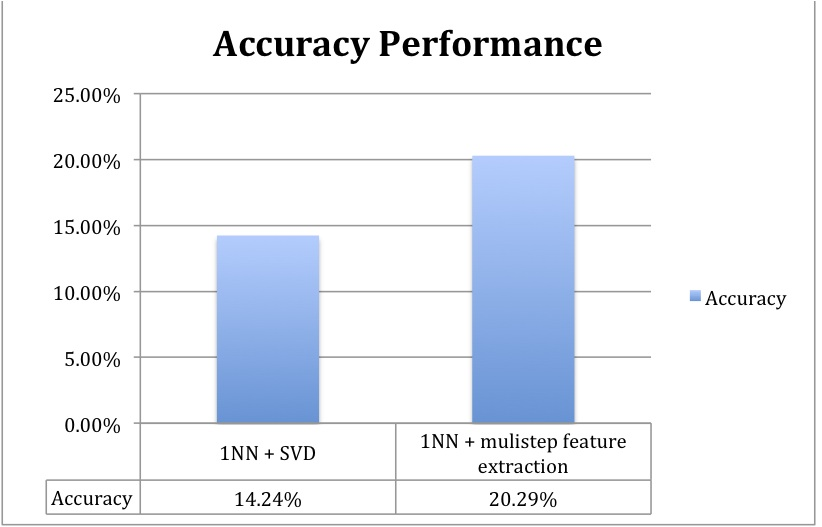
\includegraphics[scale=0.8]{84.jpg}
  \caption{Accuracy of the 1NN classifier}
   \end{figure}
  
 
\textbf{Observation}
\begin{itemize}
\item  Allowing the 1 NN classifier to exploit information about the shape of the envelopes improves the ability of  the classifier to classify intra class speech utterances more accurately by performing just a linear match between the  sequences. From figure 8.4, we can observe embedding the multi step feature extraction methodology improves the accuracy of the classifier by 6\%.

\item Applying the multistep feature extraction  as a preprocessing step, reduces the run time of the 1NN classifier. However, the preprocessing step on its own is quite time consuming. In the next chapter, I will present a detailed discussion on the pros and cons of the proposed  multi-step feature extraction method.


% One of the main drawbacks of this methodology is the fourier  feature extraction phase.  For problem domains where the use of fourier feature  extraction phase can not be avoided, the proposed multi-step feature extraction suffers from a essential drawback. While the decomposition level of applying the wavelet transform can be decided by conducting exploratory data analysis, to choose the appropriate number of fourier coefficients, we require a labelled training set.



  \end{itemize}

 \chapter{Discussion and Future Work}
This project has primarily focussed  in addressing the drawbacks associated with applying the Dynamic time warping algorithm and the Euclidean metric in time-series problem domains where minimising the run time is as important as improving the accuracy. 

\section {Summary and Future Work}

In the first 5 chapters, the focus has been primarily in improving  the  speed and accuracy of the DTW algorithm  in handling sequences that have very long lengths. In Chapter 4, we explored   domain dependent feature extraction techniques  that can  improve the performance of the baseline DTW algorithm. From the results gathered from numerous experiments, we  have observed  the DTW favours domain dependent  multivariate  feature sequences, for example the MFCC feature vectors in the case  of the TIDIGITS dataset, in  constructing optimal paths for intra class sequences which are much closer  to the diagonal regions of the cost matrix. In Chapter 5, the focus has been to improve the DTW algorithm itself. Section 7.2 proposes an alternative adaptation to the DTW algorithm  than augmenting it with window constraints  to tackle problem domains where minimising the  time complexity is of high priority. From conducting  various experiments, we have seen that the proposed adaption yields higher performance in both accuracy and run time when combined with both univariate and multivariate  features sequences. Due to the lack of time, we didn't manage to test the proposed DTW implementation in an unsupervised setting for  detecting motifs from time series sequences. For future work, it will be thus  interesting to test the proposed implementation in identifying motifs from long time series sequences  and  hence investigate how this proposed adapted version fairs against the baseline DTW algorithm augmented with the window constraint.




In the later chapters, the focus has shifted in improving the accuracy and speed  associated with using the Euclidean metric in identifying intra class sequences.  Chapter 6, investigates how SVD can be used to minimise the run time of classifiers/clustering algorithms using the Euclidean metric without any side effects  by  constructing a compact representation of time series sequences . Chapter 7  focusses in improving the accuracy of the Euclidean metric for comparing time series sequences. In section 7.1, we introduce the concept of the wavelet analysis and investigate how  the wavelet transform  can be used as feature extraction method to remove unnecessary details and preserve the  common trends of intra class sequences.  From conducting experiments on the UCR datasets, we have observed that using the wavelet transform combined with SVD as a preprocessing step improves both the accuracy and run time in identifying intra sequences that share time localised global and local trends.  In Section 7.2, the methodology is extended to improve the accuracy in using the Euclidean distance to identify sequences distinguished by their global shape. In this section, we introduce  a multi-step feature extraction methodology that combines the wavelet feature extraction process and SVD with curvature extraction techniques to construct a time series `fingerprint' for each class.  Experimental results have shown  that augmenting the baseline 1NN classifier with the proposed multi-step feature extraction process allows the Euclidean metric to be as effective as the DTW metric. However there are few issues that must be addressed regarding the implementation of  this technique:

\begin{itemize}
\item Parameter selection

When implementing the wavelet transform, choosing the appropriate wavelet coefficients is not that straight forward. For this project, I have used exploratory data analysis to decide on which level should the  wavelet decomposition  should be stopped and which wavelet  coefficients should be  considered for the problem dataset. Thus,  the success of using this feature extraction technique lies on how well the user interprets  the data through exploratory data analysis. To  automatically choose the appropriate wavelet coefficients, recently methods have been proposed \citep{Zhang2006,Qu2003} that uses the energy associated with the coefficients to choose appropriate features. For future work, it will  interesting to augment these automated methods to the wavelet feature extraction process and compare  the performance of the 1NN classifier against our current results  on the datasets we have considered so far. By comparing these new experimental results  with our current results, we can determine the usefulness of such automated wavelet feature extraction methodologies. 



Secondly, for the curve fitting phase, the smoothing parameter $\lambda$ must be set to an appropriate value to achieve a good fit.  While conducting my analysis, I have found that by visually comparing the corresponding fits, the value of  $\lambda$ can be chosen to an appropriate value that allows us to compute curvatures of the shapes of the dominant trends in the sequences.

For time series datasets where sequences  possess  long lengths even after the wavelet feature extraction process, the fourier extraction phase is used to extract the global shape of the sequences.  As I have mentioned in section 7.2, the global shape of sequence is associated with the fourier coefficients at the lower frequencies.  Hence taking the first k fourier coefficients allows the Euclidean metric to make comparisons based on the global shape of the sequences.  However, using the fourier extraction phase  provides a significant limitation. To  decide on  the correct number of fourier coefficients `k' , the 1NN classification is needed to  performed multiple times and  to choose the value k that  yields the highest accuracy. This provides a significant limitation as we need to have labelled training instances to choose k.  Hence, when we include the  fourier extraction phase  in the multi step feature extraction process,  the applicability of the multi-step  method  is reduced to  domains that are either supervised and semi-supervised.

 \item Run time :
 
 In chapter 7, we have seen that for time series classification problems where we need to include the fourier feature extraction phase in the   the multi-step method,  the overall run time incurred is much higher than the baseline method. Thus, in terms of run time, the proposed methodology is only efficient in problem scenarios where the fourier feature extraction phase is deemed not necessary.   
\end{itemize}
 And lastly in chapter 9, we investigate how this multistep feature extraction process can be extended to  extract latent features that identify speech utterances corresponding to the same lexical identity using information about the shape of their respective envelopes. The methodology proposed here also allows the Euclidean metric to be successfully applied on time series  sequences that of different lengths.
  
\section{Contributions}
This project makes two significant contributions:
\begin{itemize}
\item I have successfully developed an adaptation of the DTW algorithm that uses a specially designed kernel function to identify intra class sequences with greater accuracy and with  lesser run time in comparison to  the baseline DTW algorithm augmented with the most rigid window constraint. Thus in doing so, I have succeeded in improving the performance of the DTW algorithm in time series problem domains where minimising the run time is as equally important and improving accuracy.
\item I have successfully constructed a multi-step feature extraction scheme  that extracts  global shape descriptors of time series  sequences. Experimental results have shown that this proposed feature extraction method allows the the Euclidean metric to be as effective as the DTW metric in time series problem domains where intra class sequences  are distinguished by their global shape.
\end{itemize}
      \end{spacing}

% To be precise, each lexical identity has a acoustic signature that allows a listener to identify utterances of that word even if the utterances correspond to samples of different speakers, 
 
  
 %datasets such as the TIDIGITS where  there exists no homophonic  words, every word has a an acoustic signature that allows For example, the utterance of word `and' has different acoustic properties  than the utterance of the word 'people'.
 
 
 
     %irrespective of the fact that utterances were spoken by different speakers or in different context or both.
  
  
  %In this chapter, I will address this issues and will primarily focus 
%  \begin{itemize}
  %\item apply the proposed preprocessing method on the Tidigits data sets . However there are some issues:   \begin {enumerate}
  %\item  sequences are not of the same length
  %probable fix : i) rescale the sequences to share the same length
  			   
	%		   ii)embed 0 at the end of each sequence to make as long as the longest sequence
  %\item  the frequency is too high..hard to capture the shape of the wave due to much varation  
  %Prob fix: translate the problem to a 2D problem. Map each signal to an image and compute the shape of the image using the 4 steps as before
  %\end{enumerate}
  
  %\item Discussion---need to discuss with you on that
  
  %\item If i get time which I doubt i want to try to the test the 4 step preprocessing methodology on a different UCR dataset.
  %\end{itemize}   
     
     
     
%% ... etc ...

%%%%%%%%
%% Any appendices should go here. The appendix files should look just like the
%% chapter files.
%\appendix


\bibliographystyle{ieeetr}
 \bibliography{../../../../../Documents/mendeley/library.bib}

%% ... etc...

%% Choose your favourite bibliography style here.
%% If you want the bibliography single-spaced (which is allowed), uncomment
%% the next line.
% \singlespace

%% Specify the bibliography file. Default is thesis.bib.

% 100 is a random guess of the total number of 
%references
%% ... that's all, folks!
\end{document}
